%========================================================
\chapter[Software Testing]{\textbf{Software Testing}}
%========================================================

In this chapter, software testing and validation techniques performed on the proposed TBML
detection framework are discussed. This includes backend analytics, transaction processing pipelines, graph construction techniques in heterogeneous environments, federated
synchronization, dashboard compliance monitoring, authentication techniques, and institutional investigation operations. In particular, this chapter describes the testing workflow
conducted in the developed software system that ensures the correct operation and synchronization within the proposed analytical system.

%========================================================
\section[Testing Environment]{\textbf{Testing Environment}}
%========================================================

The testing process was conducted in a controlled development environment consisting of Python 3.11, PyTorch, PyTorch Geometric, Apache Kafka, Memgraph, PostgreSQL, and Flower federated learning services operating within isolated virtual environments created using \texttt{venv}. Frontend monitoring interfaces were implemented and validated using Next.js, TypeScript, Tailwind CSS, Prisma ORM, Zustand state management, and JWT-based authentication workflows.

The testing workflow additionally utilized Playwright-based browser automation for validating protected dashboard routes, institutional transaction workflows, STR generation pipelines, and compliance-monitoring interfaces. Database synchronization latency, transaction propagation consistency, backend API communication, and distributed fraud-inference workflows were validated under controlled institutional transaction loads to ensure reliable execution across distributed analytical environments.

%========================================================
\section[Unit Testing]{\textbf{Unit Testing}}
%========================================================

Each backend analytical service, dashboard workflow, authentication mechanism, and database synchronization component was independently tested to validate correctness, boundary handling, synchronization stability, and operational consistency before integration into the complete TBML detection framework.
%========================================================
\subsection[Unit Testing of Authentication and RBAC Module]{\textbf{Unit Testing of Authentication and RBAC Module}}
%========================================================

The authentication and role-based access control environment was independently validated to ensure secure user authentication, authorization management, middleware-driven route protection, credential verification, and institutional role isolation across banking and regulatory dashboard interfaces. The testing workflow additionally verified protected API access, invalid credential handling, unauthorized route restrictions, and role-specific dashboard rendering across distributed monitoring environments.
\renewcommand{\arraystretch}{1.3}

\begin{table}[H]
\centering
\caption{TC-001: Unit Testing of Authentication and RBAC Module}
\label{tab:auth_rbac_test}
\vspace{0.2cm}
\begin{tabular}{|p{4.2cm}|p{9cm}|}
\hline
\textbf{Serial Number of Test Case} & TC-001 \\ \hline
\textbf{Name of Test Case} & Protected Dashboard Access Validation \\ \hline
\textbf{Feature being Tested} & Authentication and Authorization Validation \\ \hline
\textbf{Description} & Validate protected route access, JWT verification, and role-based authorization \\ \hline
\textbf{Sample Input} & Invalid JWT session and unauthorized user request \\ \hline
\textbf{Expected Output} & Unauthorized access denied with authentication error response \\ \hline
\textbf{Actual Output} & Invalid sessions blocked and unauthorized users redirected successfully \\ \hline
\textbf{Remarks} & Successful test \\ \hline
\end{tabular}
\end{table}

As shown in Table~\ref{tab:auth_rbac_test}, middleware-driven session validation successfully enforced protected route isolation and role-specific dashboard authorization across institutional monitoring environments. The testing workflow validated JWT token verification, session-expiration handling, credential validation, protected API access control, and middleware-based authorization checks across banking and regulator dashboards. Invalid credentials, unauthorized API requests, expired authentication sessions, and direct access attempts to protected routes were correctly rejected using backend access-control policies before protected resources were rendered. The authentication workflow additionally verified successful role mapping for \texttt{BANK\_USER} and \texttt{ADMIN} entities to ensure secure dashboard isolation and controlled access to institutional fraud-monitoring operations.
%========================================================
\subsection[Unit Testing of Kafka Transaction Streaming]{\textbf{Unit Testing of Kafka Transaction Streaming}}
%========================================================

The Kafka transaction streaming environment was independently tested to validate asynchronous transaction publishing, real-time event synchronization, payload integrity validation, and downstream analytical communication across distributed backend services. The testing workflow additionally verified message delivery consistency, topic-based transaction propagation, malformed payload handling, and reliable synchronization between Kafka producer and consumer services operating within the proposed framework.


\begin{table}[H]
\centering
\caption{TC-002: Unit Testing of Kafka Transaction Streaming}
\label{tab:kafka_test}
\vspace{0.2cm}

\begin{tabular}{|p{4.2cm}|p{9cm}|}
\hline
\textbf{Serial Number of Test Case} & TC-002 \\ \hline
\textbf{Name of Test Case} & Publish Valid SWIFT Transaction \\ \hline
\textbf{Feature being Tested} & Kafka Event Streaming and Message Synchronization \\ \hline
\textbf{Description} & Validate transaction publishing and topic-based event synchronization \\ \hline
\textbf{Sample Input} & JSON transaction payload containing sender, receiver, amount, and trade metadata \\ \hline
\textbf{Expected Output} & Transaction published into \texttt{incoming\_swift\_messages} topic successfully \\ \hline
\textbf{Actual Output} & Transaction streamed and synchronized successfully across Kafka services \\ \hline
\textbf{Remarks} & Successful test \\ \hline
\end{tabular}
\end{table}

As shown in Table~\ref{tab:kafka_test}, the Kafka streaming module successfully validated asynchronous transaction publishing and backend event synchronization across distributed analytical services. Producer and consumer services maintained reliable message propagation and transaction consistency during continuous event-stream processing operations. Invalid payload structures, malformed transaction metadata, and incomplete financial events were correctly rejected through backend validation workflows before downstream graph-processing and fraud-inference operations were initiated.

%========================================================
\subsection[Unit Testing of Graph Construction Module]{\textbf{Unit Testing of Graph Construction Module}}
%========================================================

The heterogeneous graph-construction environment was independently tested to validate transactional node generation, relationship mapping, multi-entity graph synchronization, and Cypher-based ingestion workflows within the Memgraph analytical environment. The testing workflow additionally verified graph consistency, entity-link generation, transaction propagation accuracy, and downstream graph availability for Hybrid HGNN--LSTM analytical inference operations.

\begin{table}[H]
\centering
\caption{TC-003: Unit Testing of Graph Construction Module}
\label{tab:graph_construction_test}
\vspace{0.2cm}

\begin{tabular}{|p{4.2cm}|p{9cm}|}
\hline
\textbf{Serial Number of Test Case} & TC-003 \\ \hline
\textbf{Name of Test Case} & Heterogeneous Graph Entity Generation \\ \hline
\textbf{Feature being Tested} & Memgraph Graph Construction and Relationship Mapping \\ \hline
\textbf{Description} & Validate transactional node generation and graph relationship synchronization \\ \hline
\textbf{Sample Input} & Valid SWIFT transaction payload with account, trade, and document metadata \\ \hline
\textbf{Expected Output} & Graph nodes and transactional relationships created successfully within Memgraph \\ \hline
\textbf{Actual Output} & Heterogeneous graph entities and multi-hop relationships generated successfully \\ \hline
\textbf{Remarks} & Successful test \\ \hline
\end{tabular}
\end{table}

As shown in Table~\ref{tab:graph_construction_test}, the graph-construction workflow successfully generated heterogeneous transactional graphs within the Memgraph environment using Cypher-based ingestion and relationship-mapping operations. Graph entities including \texttt{(:Account)}, \texttt{(:Transaction)}, and \texttt{(:Document)} were correctly synchronized with transactional relationships such as \texttt{[:SENDS]}, \texttt{[:TO]}, and \texttt{[:HAS\_DOC]} during continuous event-stream processing. The testing workflow additionally validated graph consistency, entity-link integrity, and multi-hop transactional connectivity required for downstream subgraph extraction and graph-based fraud inference operations within the proposed framework.

%========================================================
\subsection[Unit Testing of STR Generation Workflow]{\textbf{Unit Testing of STR Generation Workflow}}
%========================================================

The STR generation workflow was independently tested to validate suspicious transaction report generation, compliance-record synchronization, fraud-case escalation, and regulator-side notification propagation across distributed institutional monitoring environments. The testing workflow additionally verified report persistence, transaction-metadata preservation, audit consistency, and downstream synchronization between banking dashboards and regulator-facing compliance interfaces.


\begin{table}[H]
\centering
\caption{TC-004: Unit Testing of STR Generation Workflow}
\label{tab:str_generation_test}
\vspace{0.2cm}

\begin{tabular}{|p{4.2cm}|p{9cm}|}
\hline
\textbf{Serial Number of Test Case} & TC-004 \\ \hline
\textbf{Name of Test Case} & Suspicious Transaction Report Generation \\ \hline
\textbf{Feature being Tested} & STR Generation and Compliance Synchronization \\ \hline
\textbf{Description} & Validate fraud escalation and regulator-side STR synchronization workflow \\ \hline
\textbf{Sample Input} & Fraud-classified transaction selected from institutional monitoring dashboard \\ \hline
\textbf{Expected Output} & STR record generated and synchronized into regulator compliance environment \\ \hline
\textbf{Actual Output} & STR generated, persisted, and synchronized successfully across monitoring services \\ \hline
\textbf{Remarks} & Successful test \\ \hline
\end{tabular}
\end{table}


As shown in Table~\ref{tab:str_generation_test}, the STR workflow successfully validated automated fraud-report generation, PostgreSQL audit synchronization, and regulator-side notification propagation across distributed institutional environments. Generated STR records correctly preserved transaction metadata, fraud classifications, institutional identifiers, and investigation references during downstream compliance synchronization operations. The testing workflow additionally verified successful dashboard synchronization, report persistence, and controlled propagation of suspicious transaction alerts between banking institutions and regulatory monitoring interfaces operating within the proposed framework.

%========================================================
\subsection[Unit Testing of Notification Workflow]{\textbf{Unit Testing of Notification Workflow}}
%========================================================

The notification synchronization environment was independently tested to validate fraud-alert propagation, institutional notification delivery, compliance-event synchronization, and regulator-side alert visibility across distributed monitoring interfaces. The testing workflow additionally verified notification persistence, dashboard update consistency, backend event propagation, and synchronization between banking and regulatory compliance environments during fraud escalation operations.


\begin{table}[H]
\centering
\caption{TC-005: Unit Testing of Notification Workflow}
\label{tab:notification_workflow_test}
\vspace{0.2cm}

\begin{tabular}{|p{4.2cm}|p{9cm}|}
\hline
\textbf{Serial Number of Test Case} & TC-005 \\ \hline
\textbf{Name of Test Case} & Fraud Alert and Compliance Notification Propagation \\ \hline
\textbf{Feature being Tested} & Notification Synchronization and Alert Delivery \\ \hline
\textbf{Description} & Validate fraud-alert propagation across banking and regulator monitoring environments \\ \hline
\textbf{Sample Input} & Generated STR record linked to fraud-classified transaction \\ \hline
\textbf{Expected Output} & Compliance alerts synchronized into regulator-facing dashboard interfaces \\ \hline
\textbf{Actual Output} & Fraud notifications propagated and synchronized successfully \\ \hline
\textbf{Remarks} & Successful test \\ \hline
\end{tabular}
\end{table}


As shown in Table~\ref{tab:notification_workflow_test}, he notification workflow successfully validated fraud-alert propagation, institutional investigation updates, and STR lifecycle synchronization across distributed compliance-monitoring environments. Backend event-processing services maintained reliable notification delivery and dashboard synchronization during fraud escalation operations between banking institutions and regulatory authorities. The testing workflow additionally verified notification persistence, regulator-side alert visibility, and consistent compliance-state propagation across protected monitoring interfaces operating within the proposed framework.



%========================================================
\subsection[Integration Testing]{\textbf{Integration Testing}}
%========================================================

Integration testing was conducted to validate the interaction, synchronization consistency, and workflow stability between distributed analytical services, graph-processing environments, fraud inference pipelines, dashboard-rendering systems, and regulatory compliance workflows operating within the proposed TBML detection framework.

%========================================================
\subsection[Integration Testing of Kafka and Memgraph Pipeline]{\textbf{Integration Testing of Kafka and Memgraph Pipeline}}
%========================================================

This integration test validated end-to-end synchronization between Kafka-based transaction streaming services and the heterogeneous graph-construction environment operating within Memgraph. The testing workflow additionally verified event-stream consistency, transaction propagation reliability, graph-ingestion stability, and downstream synchronization between distributed backend services.

\renewcommand{\arraystretch}{1.3}

\begin{table}[H]
\centering
\caption{TC-006: Integration Testing of Kafka and Memgraph Pipeline}
\label{tab:kafka_memgraph_integration_test}`'
\vspace{0.2cm}

\begin{tabular}{|p{4.2cm}|p{9cm}|}
\hline
\textbf{Serial Number of Test Case} & TC-006 \\ \hline
\textbf{Name of Test Case} & Transaction Stream and Graph Synchronization Workflow \\ \hline
\textbf{Feature being Tested} & Kafka Event Propagation and Memgraph Synchronization \\ \hline
\textbf{Description} & Validate transaction-stream synchronization and heterogeneous graph generation \\ \hline
\textbf{Sample Input} & Valid Kafka transaction payload with trade metadata and KYC attributes \\ \hline
\textbf{Expected Output} & Transactional graph entities and relationships generated successfully within Memgraph \\ \hline
\textbf{Actual Output} & Kafka events synchronized and heterogeneous graph generated successfully \\ \hline
\textbf{Remarks} & Successful test \\ \hline
\end{tabular}
\end{table}

\renewcommand{\arraystretch}{1}

As shown in Table~\ref{tab:kafka_memgraph_integration_test}, the integration workflow successfully validated asynchronous transaction propagation between Kafka producer-consumer services and Memgraph graph-ingestion environments. Streamed SWIFT transaction events were reliably synchronized into graph-processing pipelines without transactional inconsistency or event-loss during continuous backend processing operations. The testing workflow additionally verified stable graph synchronization, multi-entity relationship generation, and downstream availability of transactional subgraphs required for graph-based analytical inference within the proposed framework.


%========================================================
\subsection[Integration Testing of Fraud Prediction and Dashboard Synchronization]{\textbf{Integration Testing of Fraud Prediction and Dashboard Synchronization}}
%========================================================

This integration test validated synchronization between fraud-prediction services, PostgreSQL audit environments, and role-based monitoring dashboards operating within the proposed TBML framework. The testing workflow additionally verified database persistence, dashboard synchronization consistency, and real-time rendering of fraud-classified transactions.

\renewcommand{\arraystretch}{1.3}

\begin{table}[H]
\centering
\caption{TC-007: Integration Testing of Fraud Prediction and Dashboard Synchronization}
\label{tab:fraud_prediction_dashboard_integration_test}
\vspace{0.2cm}

\begin{tabular}{|p{4.2cm}|p{9cm}|}
\hline
\textbf{Serial Number of Test Case} & TC-007 \\ \hline
\textbf{Name of Test Case} & Fraud Prediction and Dashboard Rendering Workflow \\ \hline
\textbf{Feature being Tested} & PostgreSQL Synchronization and Dashboard Visualization \\ \hline
\textbf{Description} & Validate fraud-prediction synchronization into institutional monitoring dashboards \\ \hline
\textbf{Sample Input} & Fraud-classified transaction generated from analytical inference pipeline \\ \hline
\textbf{Expected Output} & Fraud transaction persisted and rendered successfully within dashboard interfaces \\ \hline
\textbf{Actual Output} & Dashboard synchronization completed successfully with valid fraud-state rendering \\ \hline
\textbf{Remarks} & Successful test \\ \hline
\end{tabular}
\end{table}

\renewcommand{\arraystretch}{1}

The integration test ensured proper synchronization of fraud-prediction services,
PostgreSQL audit environments, and dashboards for role-based monitoring working
under the TBML architecture. The testing process further confirmed persistence of the
database, consistency of dashboard synchronization, and rendering of fraud-classified
transactions.  Integration Testing of Fraud Prediction and Dashboard Synchronization It can be seen from Table~\ref{tab:fraud_prediction_dashboard_integration_test} that records of fraud predictions, transaction data, and
risk classifications of institutions were synchronized in centralized PostgreSQL audit
systems and then rendered using secure dashboard applications. The synchronization of the dashboards ensured proper propagation of fraud status and transaction visibility in
institutional monitoring services.


%========================================================
\subsection[Integration Testing of STR Generation Workflow]{\textbf{Integration Testing of STR Generation Workflow}}
%========================================================
This integration test confirmed the full integration from institutional fraud verification, STR generation services, regulator-side synchronization and propagation of compliance notifications in the distributed monitoring environments. The testing process also confirmed that fraud escalation is consistent, reports are persistent, and regulators are seamlessly visible throughout institutional compliance workflows.

The STR synchronization workflow was successfully tested in institutional monitoring environments for fraud escalation, generation of compliance reports, synchronization of the Regulator side dashboard, and propagation of notifications. Downstream fraud processing compliance operations were consistently able to maintain fraud types, investigation metadata, identifiers for institutions and audit references in generated STR records. The testing workflow also confirmed that compliance data could be propagated successfully to compliance monitoring interfaces and that suspicious transaction reports could be propagated and viewed across banking and regulatory interfaces, as shown in Table~\ref{tab:str_generation_integration_test}.

\renewcommand{\arraystretch}{1.3}

\begin{table}[H]
\centering
\caption{TC-008: Integration Testing of STR Generation Workflow}
\label{tab:str_generation_integration_test}
\vspace{0.2cm}

\begin{tabular}{|p{4.2cm}|p{9cm}|}
\hline
\textbf{Serial Number of Test Case} & TC-008 \\ \hline
\textbf{Name of Test Case} & Fraud Escalation and STR Compliance Workflow \\ \hline
\textbf{Feature being Tested} & STR Lifecycle Management and Compliance Synchronization \\ \hline
\textbf{Description} & Validate fraud escalation and regulator-side STR synchronization workflow \\ \hline
\textbf{Sample Input} & Fraud transaction escalated by institutional administrator \\ \hline
\textbf{Expected Output} & STR generated and synchronized successfully within regulator compliance dashboard \\ \hline
\textbf{Actual Output} & Fraud escalation and STR synchronization completed successfully \\ \hline
\textbf{Remarks} & Successful test \\ \hline
\end{tabular}
\end{table}

\renewcommand{\arraystretch}{1}

%========================================================
\subsection[Integration Testing of Authentication and Protected Dashboard Rendering]{\textbf{Integration Testing of Authentication and Protected Dashboard Rendering}}
%========================================================

This integration test validated synchronization between JWT-based authentication services, middleware-driven authorization guards, protected API routes, and role-specific dashboard-rendering environments operating within the proposed framework. The testing workflow additionally verified secure session propagation, authorization consistency, and protected resource accessibility across institutional monitoring interfaces.

Middleware-driven authentication workflows successfully validated session authorization, protected route synchronization, secure API accessibility, and institutional role isolation across distributed monitoring interfaces. Dashboard-rendering operations correctly enforced role-specific access-control policies for \texttt{BANK\_USER}, \texttt{ADMIN}, and \texttt{REGULATOR} entities during backend synchronization workflows. The testing workflow additionally verified invalid-session rejection, unauthorized route restrictions, and secure propagation of authenticated dashboard resources across institutional compliance-monitoring environments. The corresponding test results are summarized in Table~\ref{tab:auth_dashboard_integration_test}.
\renewcommand{\arraystretch}{1.3}

\begin{table}[H]
\centering
\caption{TC-009: Integration Testing of Authentication and Protected Dashboard Rendering}
\label{tab:auth_dashboard_integration_test}
\vspace{0.2cm}

\begin{tabular}{|p{4.2cm}|p{9cm}|}
\hline
\textbf{Serial Number of Test Case} & TC-009 \\ \hline
\textbf{Name of Test Case} & Authenticated Dashboard Access and Rendering Workflow \\ \hline
\textbf{Feature being Tested} & Session Validation and Role-Based Dashboard Authorization \\ \hline
\textbf{Description} & Validate authenticated dashboard rendering and protected route authorization \\ \hline
\textbf{Sample Input} & Valid JWT-authenticated institutional user session \\ \hline
\textbf{Expected Output} & Authorized dashboard rendered successfully based on institutional role \\ \hline
\textbf{Actual Output} & Protected dashboard rendered successfully with valid role authorization \\ \hline
\textbf{Remarks} & Successful test \\ \hline
\end{tabular}
\end{table}

\renewcommand{\arraystretch}{1}

%========================================================
\section[System Testing]{\textbf{System Testing}}
%========================================================

System testing was conducted to validate the operational stability, concurrent transaction-handling capability, database synchronization performance, and workflow-level response consistency of the proposed TBML detection framework under distributed institutional monitoring environments. The testing workflow focused on browser-based end-to-end validation, protected dashboard execution, concurrent PostgreSQL scalability analysis, API response-time benchmarking, and operational latency evaluation across fraud-monitoring and compliance-management services.

%========================================================
\subsection[Browser Automation and Workflow Validation]{\textbf{Browser Automation and Workflow Validation}}
%========================================================

Browser-based end-to-end validation was performed using Playwright automation workflows executed within Chromium testing environments. The testing workflow validated protected dashboard rendering, role-based authentication, STR lifecycle execution, fraud-notification propagation, compliance-action synchronization, and institutional transaction visibility restrictions across distributed frontend and backend services. All automated workflow executions completed successfully without unauthorized access, synchronization failure, or dashboard inconsistency during operational validation.

The Playwright automation workflow was able to validate sequential execution of institutional fraud-monitoring operations in protected dashboard environments. Browser automation also validated persistent sessions, API synchronization consistency, authorization level validation at the workflow level, and consistent dashboard rendering for both the \texttt{ADMIN} and \texttt{BANK\_USER} operational environments. The testing workflow also demonstrated successful generation of STR, fraud escalation, compliance synchronization, and propagation of notifications across automated end-to-end workflows. Summary of the workflow validation results for browsers is summarized in Table~\ref{tab:browser_automation_test}.
\renewcommand{\arraystretch}{1.3}

\begin{table}[H]
\centering
\caption{TC-010: Browser Automation and Workflow Validation Results}
\label{tab:browser_automation_test}
\vspace{0.2cm}

\begin{tabular}{|p{7cm}|p{4cm}|}
\hline
\textbf{Workflow Validation} & \textbf{Status} \\ \hline
Admin Authentication and Dashboard Rendering & Successful \\ \hline
Fraud Case Retrieval and STR Visibility & Successful \\ \hline
GET\_DOCUMENTS Compliance Workflow & Successful \\ \hline
FREEZE\_ACCOUNT Regulatory Workflow & Successful \\ \hline
Fraud Verdict Marking Workflow & Successful \\ \hline
Bank User STR Generation Workflow & Successful \\ \hline
Fraud Notification Propagation Workflow & Successful \\ \hline
Protected Route and RBAC Validation & Successful \\ \hline
Institutional Transaction Visibility Restriction & Successful \\ \hline
Sign-In Page Smoke Testing & Successful \\ \hline
\end{tabular}
\end{table}

\renewcommand{\arraystretch}{1}

%========================================================
\subsection[Concurrent Database Scalability and API Performance Analysis]{\textbf{Concurrent Database Scalability and API Performance Analysis}}
%========================================================
To assess PostgreSQL synchronization stability, dashboard query performance, fraud-filtering latency and the consistency of STR retrieval responses in the presence of growing loads of institutional users, concurrent database scalability testing was performed. To achieve this, the benchmarking workflow has been developed to run on Prisma ORM and Next.js backend services, with each institutional user simulator performing five sequential transactional requests while performing concurrent operations accessing the dashboard. To ensure that the maximum simultaneous connections to the backend will be limited to 15, the controlled concurrency execution used batched asynchronous request propagation with pooled PostgreSQL database connections in order to control the synchronization of transactions, avoid backend resource exhaustion and guarantee the behavior of queries being executed during high volume monitoring workloads.

Latency benchmarking was done by taking the time taken to initiate a request and time taken to receive the response while running concurrent execution of the API. The benchmarking workflow captured the time of the request call with \texttt{startTime = performance.now()}, then asynchronous API call was executed and the backend response was synchronized. The response-completion timestamp was marked as startTime = performance.now() in the transactional request and endTime = performance.now() after successful completion of the transactional request and the operational latency computed as latency = endTime - startTime. The software included concurrent workload execution, achieved via parallel asynchronous request propagation, which involved multiple simulated institutional users running concurrent operations on dashboard and compliance-query applications at a controlled concurrency level.

Average latency data was measured as the average response time of all the successful transactional calls, and P95 latency data was measured as the upper bound latency response when the synchronization is at its peak. The benchmarking workflow also tested distantly deployed compliance-monitoring environments for request throughput, API synchronization consistency, transaction persistence reliability, and consistent PostgreSQL query execution.

These operational latency equations were used to calculate the benchmarking metrics:
\begin{equation}
L_{\text{avg}} =
\frac{1}{N}
\sum_{i=1}^{N}
(T_{\text{response}_i} - T_{\text{request}_i})
\end{equation}

\begin{equation}
L_{95} =
\operatorname{Percentile}_{95}(L_1, L_2, \dots, L_N)
\end{equation}

\renewcommand{\arraystretch}{1.3}

\begin{table}[H]
\centering
\caption{TC-011: Dashboard Transaction Retrieval Scalability Analysis}
\label{tab:dashboard_transaction_retrieval_scalability_test}
\vspace{0.2cm}

\begin{tabular}{|p{2.6cm}|p{2.4cm}|p{2.8cm}|p{2.8cm}|p{2.2cm}|}
\hline
\textbf{Concurrent Users} & \textbf{Total Requests} & \textbf{Avg Latency (ms)} & \textbf{P95 Latency (ms)} & \textbf{Success Rate} \\ \hline
10 & 50 & 297.33 & 884.28 & 100\% \\ \hline
50 & 250 & 156.05 & 174.75 & 100\% \\ \hline
100 & 500 & 159.99 & 181.30 & 100\% \\ \hline
250 & 1250 & 158.53 & 176.99 & 100\% \\ \hline
500 & 2500 & 162.14 & 180.72 & 100\% \\ \hline
\end{tabular}
\end{table}

\renewcommand{\arraystretch}{1}

As shown in Table~\ref{tab:dashboard_transaction_retrieval_scalability_test}, the dashboard transaction retrieval workflow demonstrated stable query scalability and consistent dashboard-rendering performance across increasing institutional user loads. Average latency values remained nearly constant between 50 and 500 concurrent users, indicating efficient PostgreSQL query execution, optimized transactional indexing, and stable backend synchronization during high-frequency dashboard-access operations. The relatively low variation between average and P95 latency measurements further indicated predictable response behavior and controlled query-execution overhead under concurrent transactional workloads.

\renewcommand{\arraystretch}{1.3}

\begin{table}[H]
\centering
\caption{TC-012: Fraud Transaction Filtering Scalability Analysis}
\label{tab:fraud_transaction_filtering_scalability_test}
\vspace{0.2cm}

\begin{tabular}{|p{2.6cm}|p{2.4cm}|p{2.8cm}|p{2.8cm}|p{2.2cm}|}
\hline
\textbf{Concurrent Users} & \textbf{Total Requests} & \textbf{Avg Latency (ms)} & \textbf{P95 Latency (ms)} & \textbf{Success Rate} \\ \hline
10 & 50 & 159.58 & 174.04 & 100\% \\ \hline
50 & 250 & 158.15 & 181.58 & 100\% \\ \hline
100 & 500 & 147.56 & 170.37 & 100\% \\ \hline
250 & 1250 & 148.18 & 164.58 & 100\% \\ \hline
500 & 2500 & 263.80 & 731.88 & 100\% \\ \hline
\end{tabular}
\end{table}

\renewcommand{\arraystretch}{1}

As shown in Table~\ref{tab:fraud_transaction_filtering_scalability_test}, the fraud-transaction filtering workflow demonstrated efficient analytical-query execution and stable institution-specific transaction retrieval during concurrent dashboard operations. Lower average latency values under moderate workloads indicated optimized fraud-state filtering and indexed transactional query execution across backend analytical services. Increased P95 latency under 500-user workloads indicated temporary synchronization overhead during peak concurrent analytical filtering operations; however, the framework maintained complete request reliability, stable API synchronization, and consistent fraud-state propagation throughout distributed monitoring workflows.

\renewcommand{\arraystretch}{1.3}

\begin{table}[H]
\centering
\caption{TC-013: STR Compliance Report Retrieval Scalability Analysis}
\label{tab:str_compliance_report_retrieval_scalability_test}
\vspace{0.2cm}

\begin{tabular}{|p{2.6cm}|p{2.4cm}|p{2.8cm}|p{2.8cm}|p{2.2cm}|}
\hline
\textbf{Concurrent Users} & \textbf{Total Requests} & \textbf{Avg Latency (ms)} & \textbf{P95 Latency (ms)} & \textbf{Success Rate} \\ \hline
10 & 50 & 2694.21 & 7311.50 & 100\% \\ \hline
50 & 250 & 2101.61 & 4791.52 & 100\% \\ \hline
100 & 500 & 856.39 & 2149.27 & 100\% \\ \hline
250 & 1250 & 467.03 & 600.67 & 100\% \\ \hline
500 & 2500 & 465.62 & 596.76 & 100\% \\ \hline
\end{tabular}
\end{table}

\renewcommand{\arraystretch}{1}

As shown in Table~\ref{tab:str_compliance_report_retrieval_scalability_test}, the STR compliance retrieval workflow exhibited comparatively higher latency due to compliance-report aggregation, transaction-history synchronization, regulator-side metadata retrieval, and multi-table relational query execution during report-generation operations. However, the gradual reduction in average latency under increasing concurrent workloads indicated improved PostgreSQL query stabilization, efficient pooled connection utilization, and optimized relational-query execution during sustained processing operations.

Despite the additional computational overhead associated with compliance-report generation, the framework maintained stable request consistency and complete request success rates across distributed monitoring environments. The testing workflows validated reliable backend synchronization, controlled API response behavior, stable federated analytical execution, and consistent PostgreSQL query performance under increasing institutional workloads.


The conducted testing workflows validated the synchronization reliability, operational stability, and execution consistency of the proposed TBML detection framework across distributed monitoring environments. The testing results confirmed stable backend communication, reliable transactional synchronization, controlled API response behavior, and successful workflow execution across graph-processing, federated analytical inference, dashboard synchronization, and compliance-management services. Concurrent scalability validation additionally demonstrated stable PostgreSQL query execution and controlled latency characteristics under increasing institutional workloads.



%========================================================
\section[Model Performance Evaluation]{\textbf{Model Performance Evaluation}}
%========================================================

The proposed federated Hybrid HGNN--LSTM framework was evaluated across three distributed institutional clients (BANKA, BANKB, and BANKC) to validate fraud-classification capability and federated convergence stability across heterogeneous transactional environments. Multi-class prediction performance for \textit{Clean}, \textit{Watchlist}, and \textit{Fraud} transaction states was analyzed using Precision, Recall, F1-Score, confusion-matrix validation, and Precision--Recall benchmarking. Federated parameter synchronization was performed using the FedAvg aggregation strategy across 10 federated communication rounds.

The transactional dataset was partitioned using a stratified temporal split strategy to preserve chronological separation between training and testing samples while maintaining balanced representation across minority fraud categories. Weighted cross-entropy optimization and gradient clipping mechanisms were integrated to stabilize distributed training and address fraud-class imbalance during federated convergence operations. Precision--Recall evaluation was prioritized over standalone classification accuracy due to the highly imbalanced nature of illicit transactional behavior within institutional financial environments.

%========================================================
\subsection[Multi-Class Classification Performance]{\textbf{Multi-Class Classification Performance}}
%========================================================

The final federated classification results obtained after 10 federated aggregation rounds across all participating institutional environments are summarized in Table~\ref{tab:model_performance}. The evaluation was conducted to analyze the framework’s ability to distinguish legitimate, suspicious, and fraudulent transactional behaviors across distributed institutional datasets under federated learning conditions. The obtained results additionally validated stable analytical convergence and consistent fraud-classification performance across all participating banking clients.


The evaluation results demonstrated stable multi-class classification performance across all distributed institutional clients. Clean transactional states achieved near-perfect Precision and Recall, thereby minimizing false-positive propagation during large-scale monitoring operations. The Watchlist class maintained Recall values above $0.97$, indicating effective identification of suspicious transactional behavior requiring institutional review workflows.

\begin{table}[H]
\centering
\caption{Federated Multi-Class Classification Performance result}
\vspace{0.3cm}

\renewcommand{\arraystretch}{1.3}

\begin{tabular}{|p{2.2cm}|p{3cm}|p{2cm}|p{2cm}|p{2cm}|}
\hline
\textbf{Institution} & \textbf{Transaction Class} & \textbf{Precision} & \textbf{Recall} & \textbf{F1-Score} \\ \hline

\multirow{3}{*}{BANKA}
& Clean (0) & 1.00 & 1.00 & 1.00 \\ \cline{2-5}
& Watchlist (1) & 0.79 & 0.97 & 0.87 \\ \cline{2-5}
& Fraud (2) & 0.96 & 0.73 & 0.83 \\ \hline

\multirow{3}{*}{BANKB}
& Clean (0) & 1.00 & 1.00 & 1.00 \\ \cline{2-5}
& Watchlist (1) & 0.79 & 0.99 & 0.88 \\ \cline{2-5}
& Fraud (2) & 0.98 & 0.73 & 0.84 \\ \hline

\multirow{3}{*}{BANKC}
& Clean (0) & 1.00 & 1.00 & 1.00 \\ \cline{2-5}
& Watchlist (1) & 0.79 & 0.99 & 0.88 \\ \cline{2-5}
& Fraud (2) & 0.98 & 0.73 & 0.84 \\ \hline

\end{tabular}

\renewcommand{\arraystretch}{1}

\label{tab:model_performance}
\end{table}


The accuracy of fraud predictions was between $0.96$ and $0.98$; this result is good to know, since transactional activity that is identified as fraud is identified correctly, and only a small number of false fraud escalations occur. The framework maintained robust fraud-discrimination capability while Facepoker's Recall remained near $0.73$ despite very skewed distributions of transactions and complicated multi-hop laundering structures. The resulting F1-scores also confirm that there is a good balance between the accuracy of fraud detection and the consistency of classification for all the participating institutions. The results of BANKA, BANKB and BANKC are fairly similar, showing that the federated training method is effective in learning generalised fraud patterns in distributed transactional environments. In sum, the results confirm stable federated generalization and strong analytical capabilities without the need for centralized access to sensitive financial data to detect TBML, thus enabling privacy-preserving and collaborative TBML detection.

%========================================================
\subsection[Federated Convergence Analysis]{\textbf{Federated Convergence Analysis}}
%========================================================

Longitudinal Accuracy, Precision and Recall progression analysis was used to evaluate the federated convergence workflow in the iterative federated aggregation rounds. The convergence curves were generated independently for all the institutional clients to validate the consistency of distributed synchronization and global-weight stabilization in the federated optimization workflows.
%--------------------------------------------------------
\subsection{BANKA Federated Convergence}
%--------------------------------------------------------
\begin{figure}[H]
\centering

% Top Row
\begin{minipage}{0.48\textwidth}
\centering
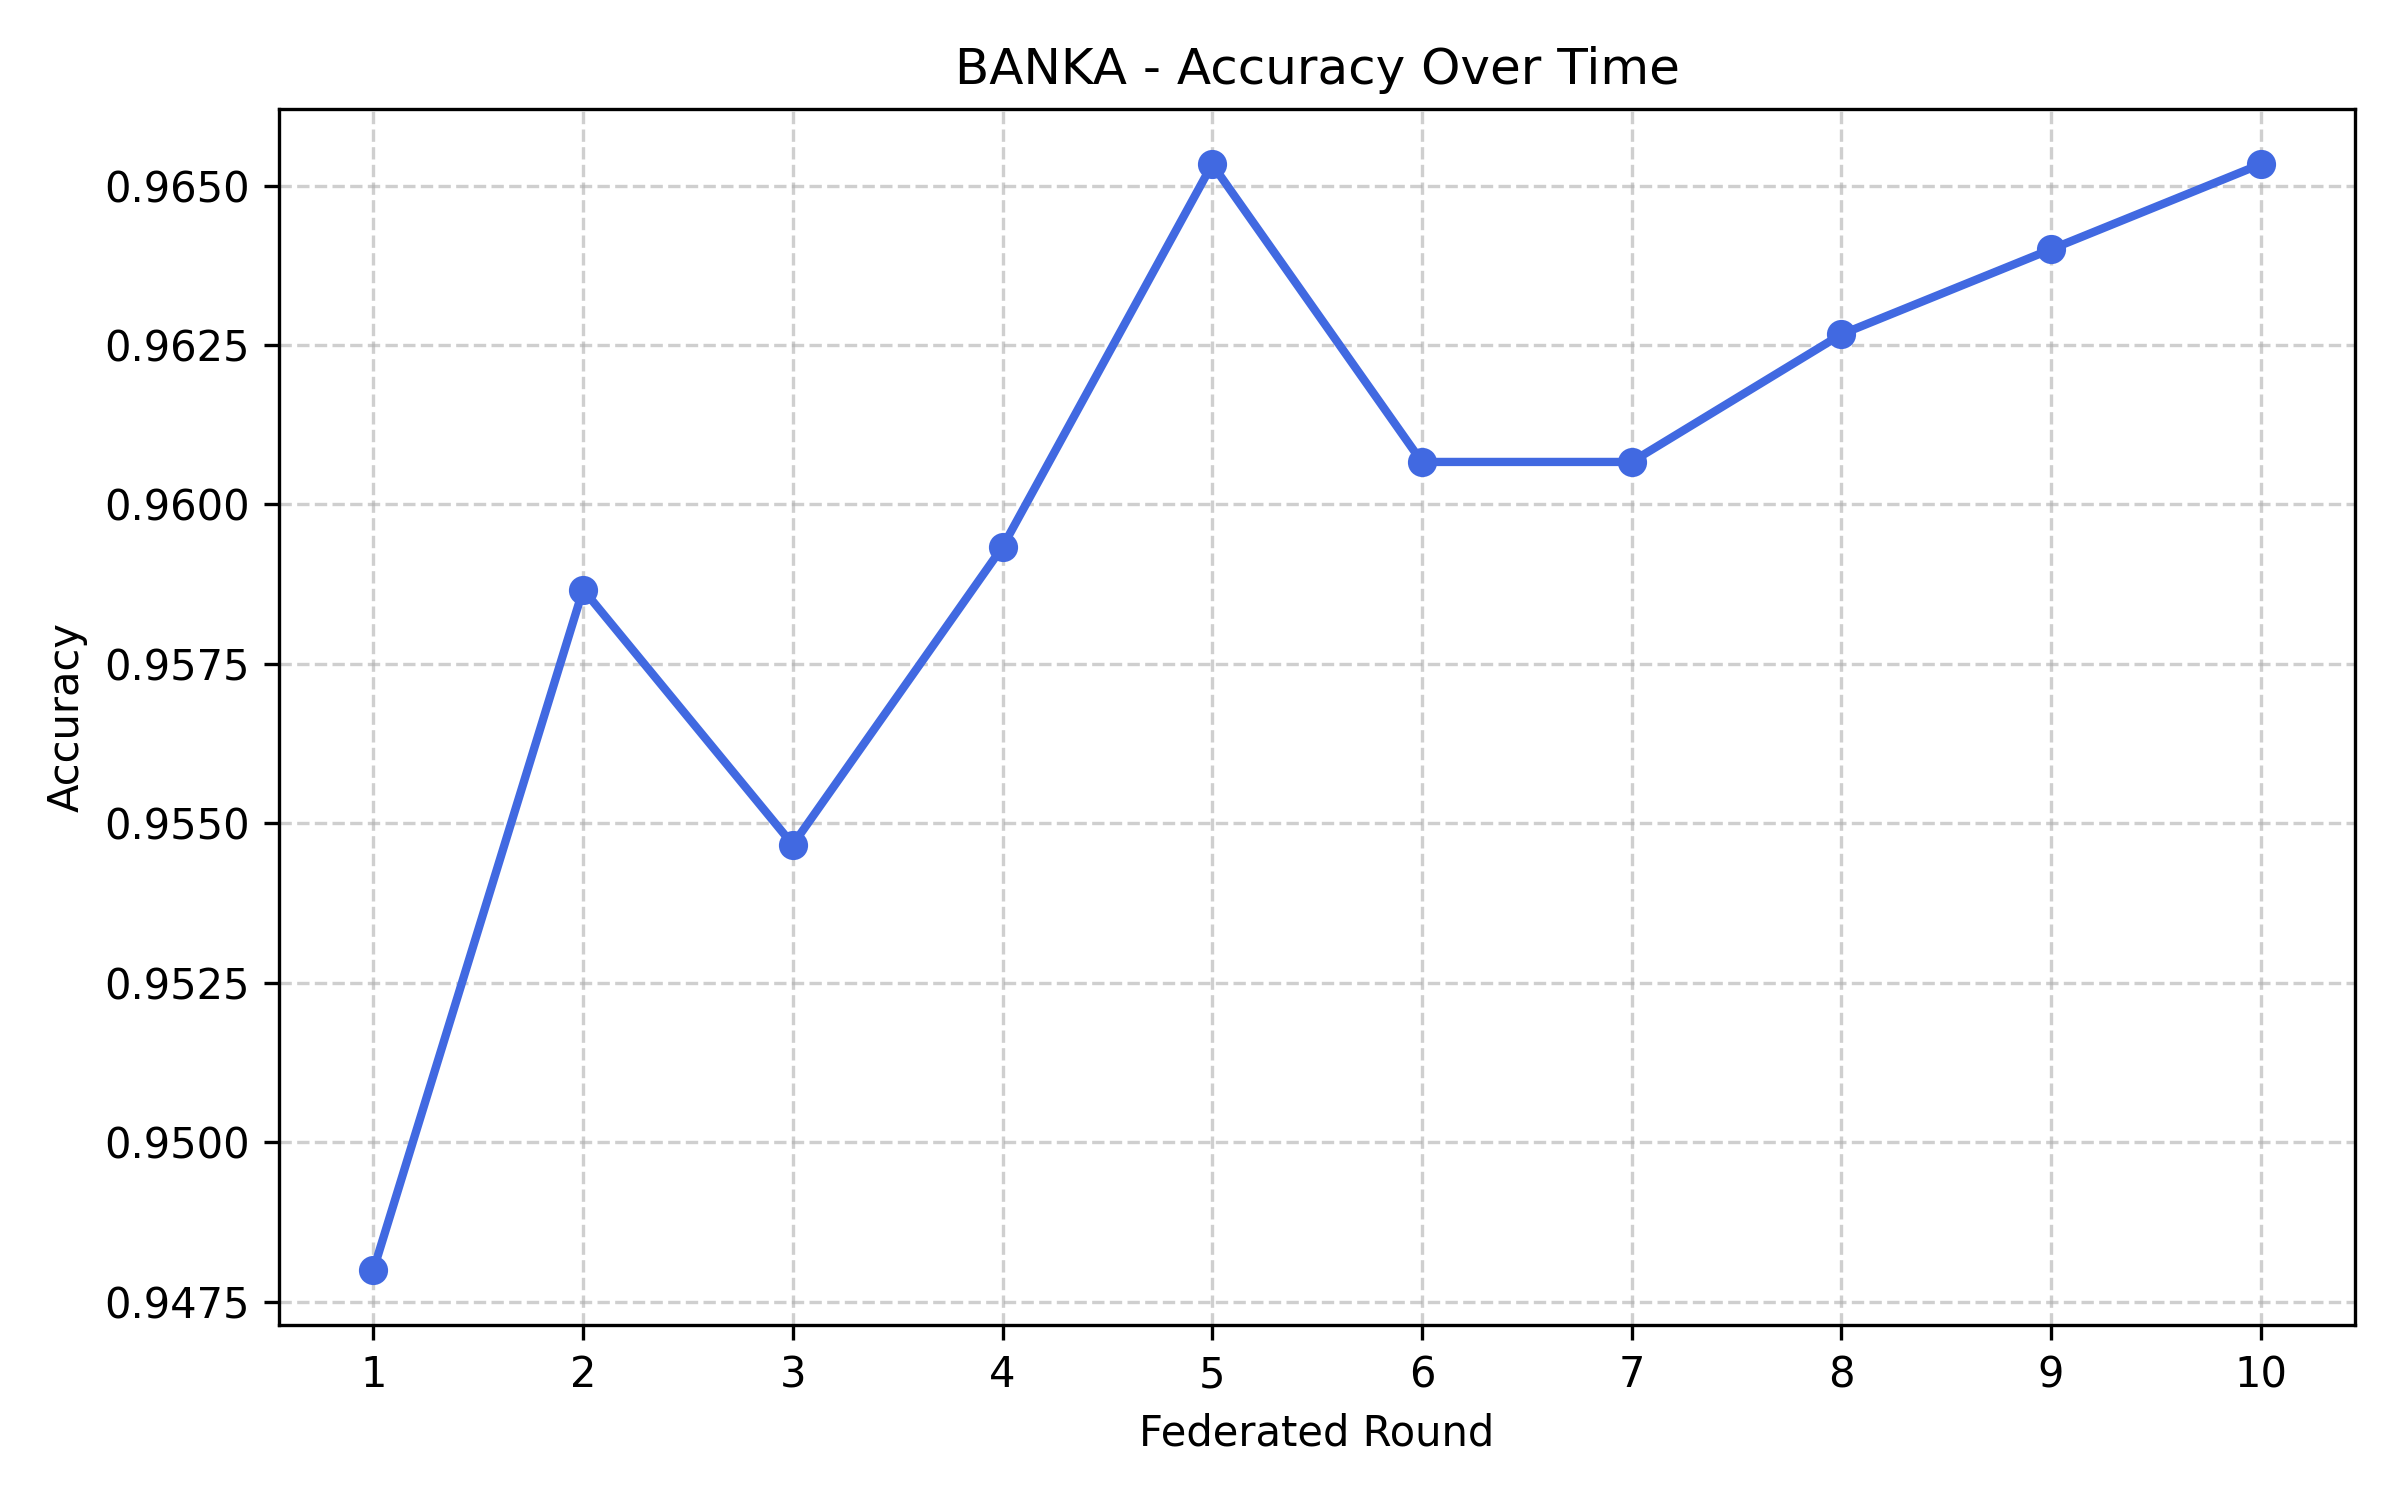
\includegraphics[width=\linewidth]{Figures/banka_progression_accuracy.png}

\vspace{0.1cm}
{\small (a) BANKA Accuracy vs Federated Aggregation Rounds}\end{minipage}
\hfill
\begin{minipage}{0.48\textwidth}
\centering
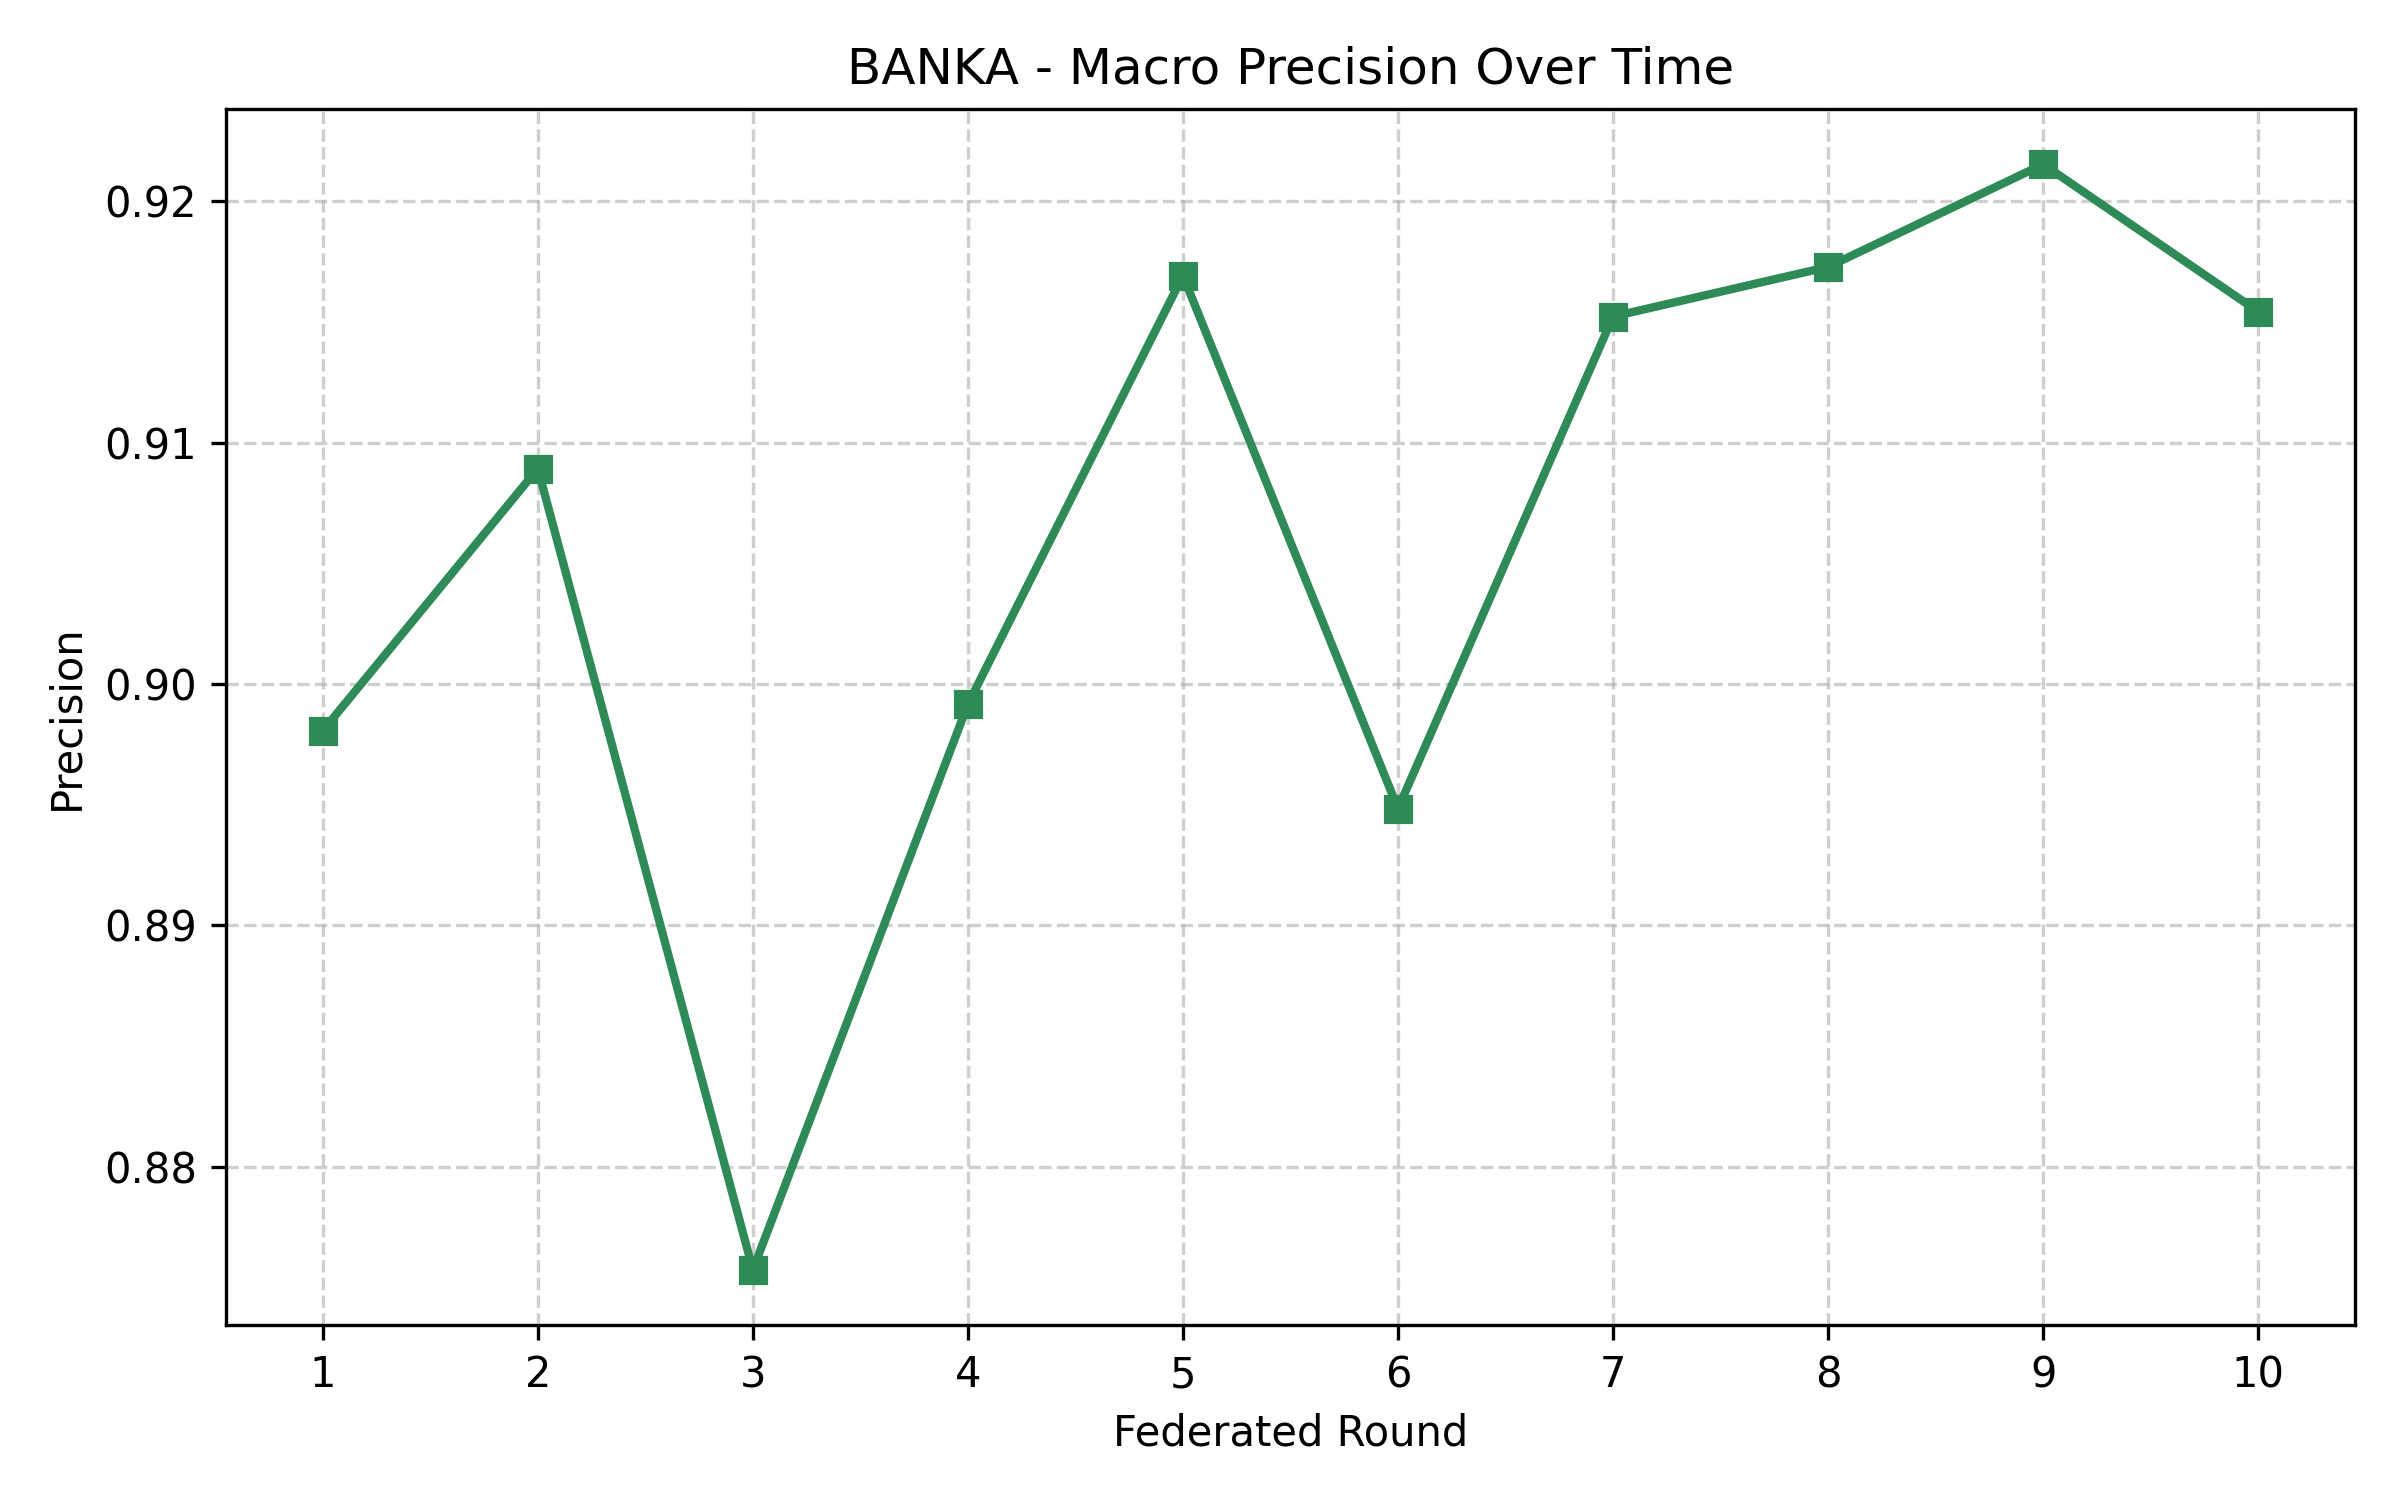
\includegraphics[width=\linewidth]{Figures/banka_progression_precision.png}

\vspace{0.1cm}
{\small (b) BANKA Precision vs Federated Aggregation Rounds}\end{minipage}
\vspace{0.4cm}

% Bottom Row
\begin{minipage}{0.48\textwidth}
\centering
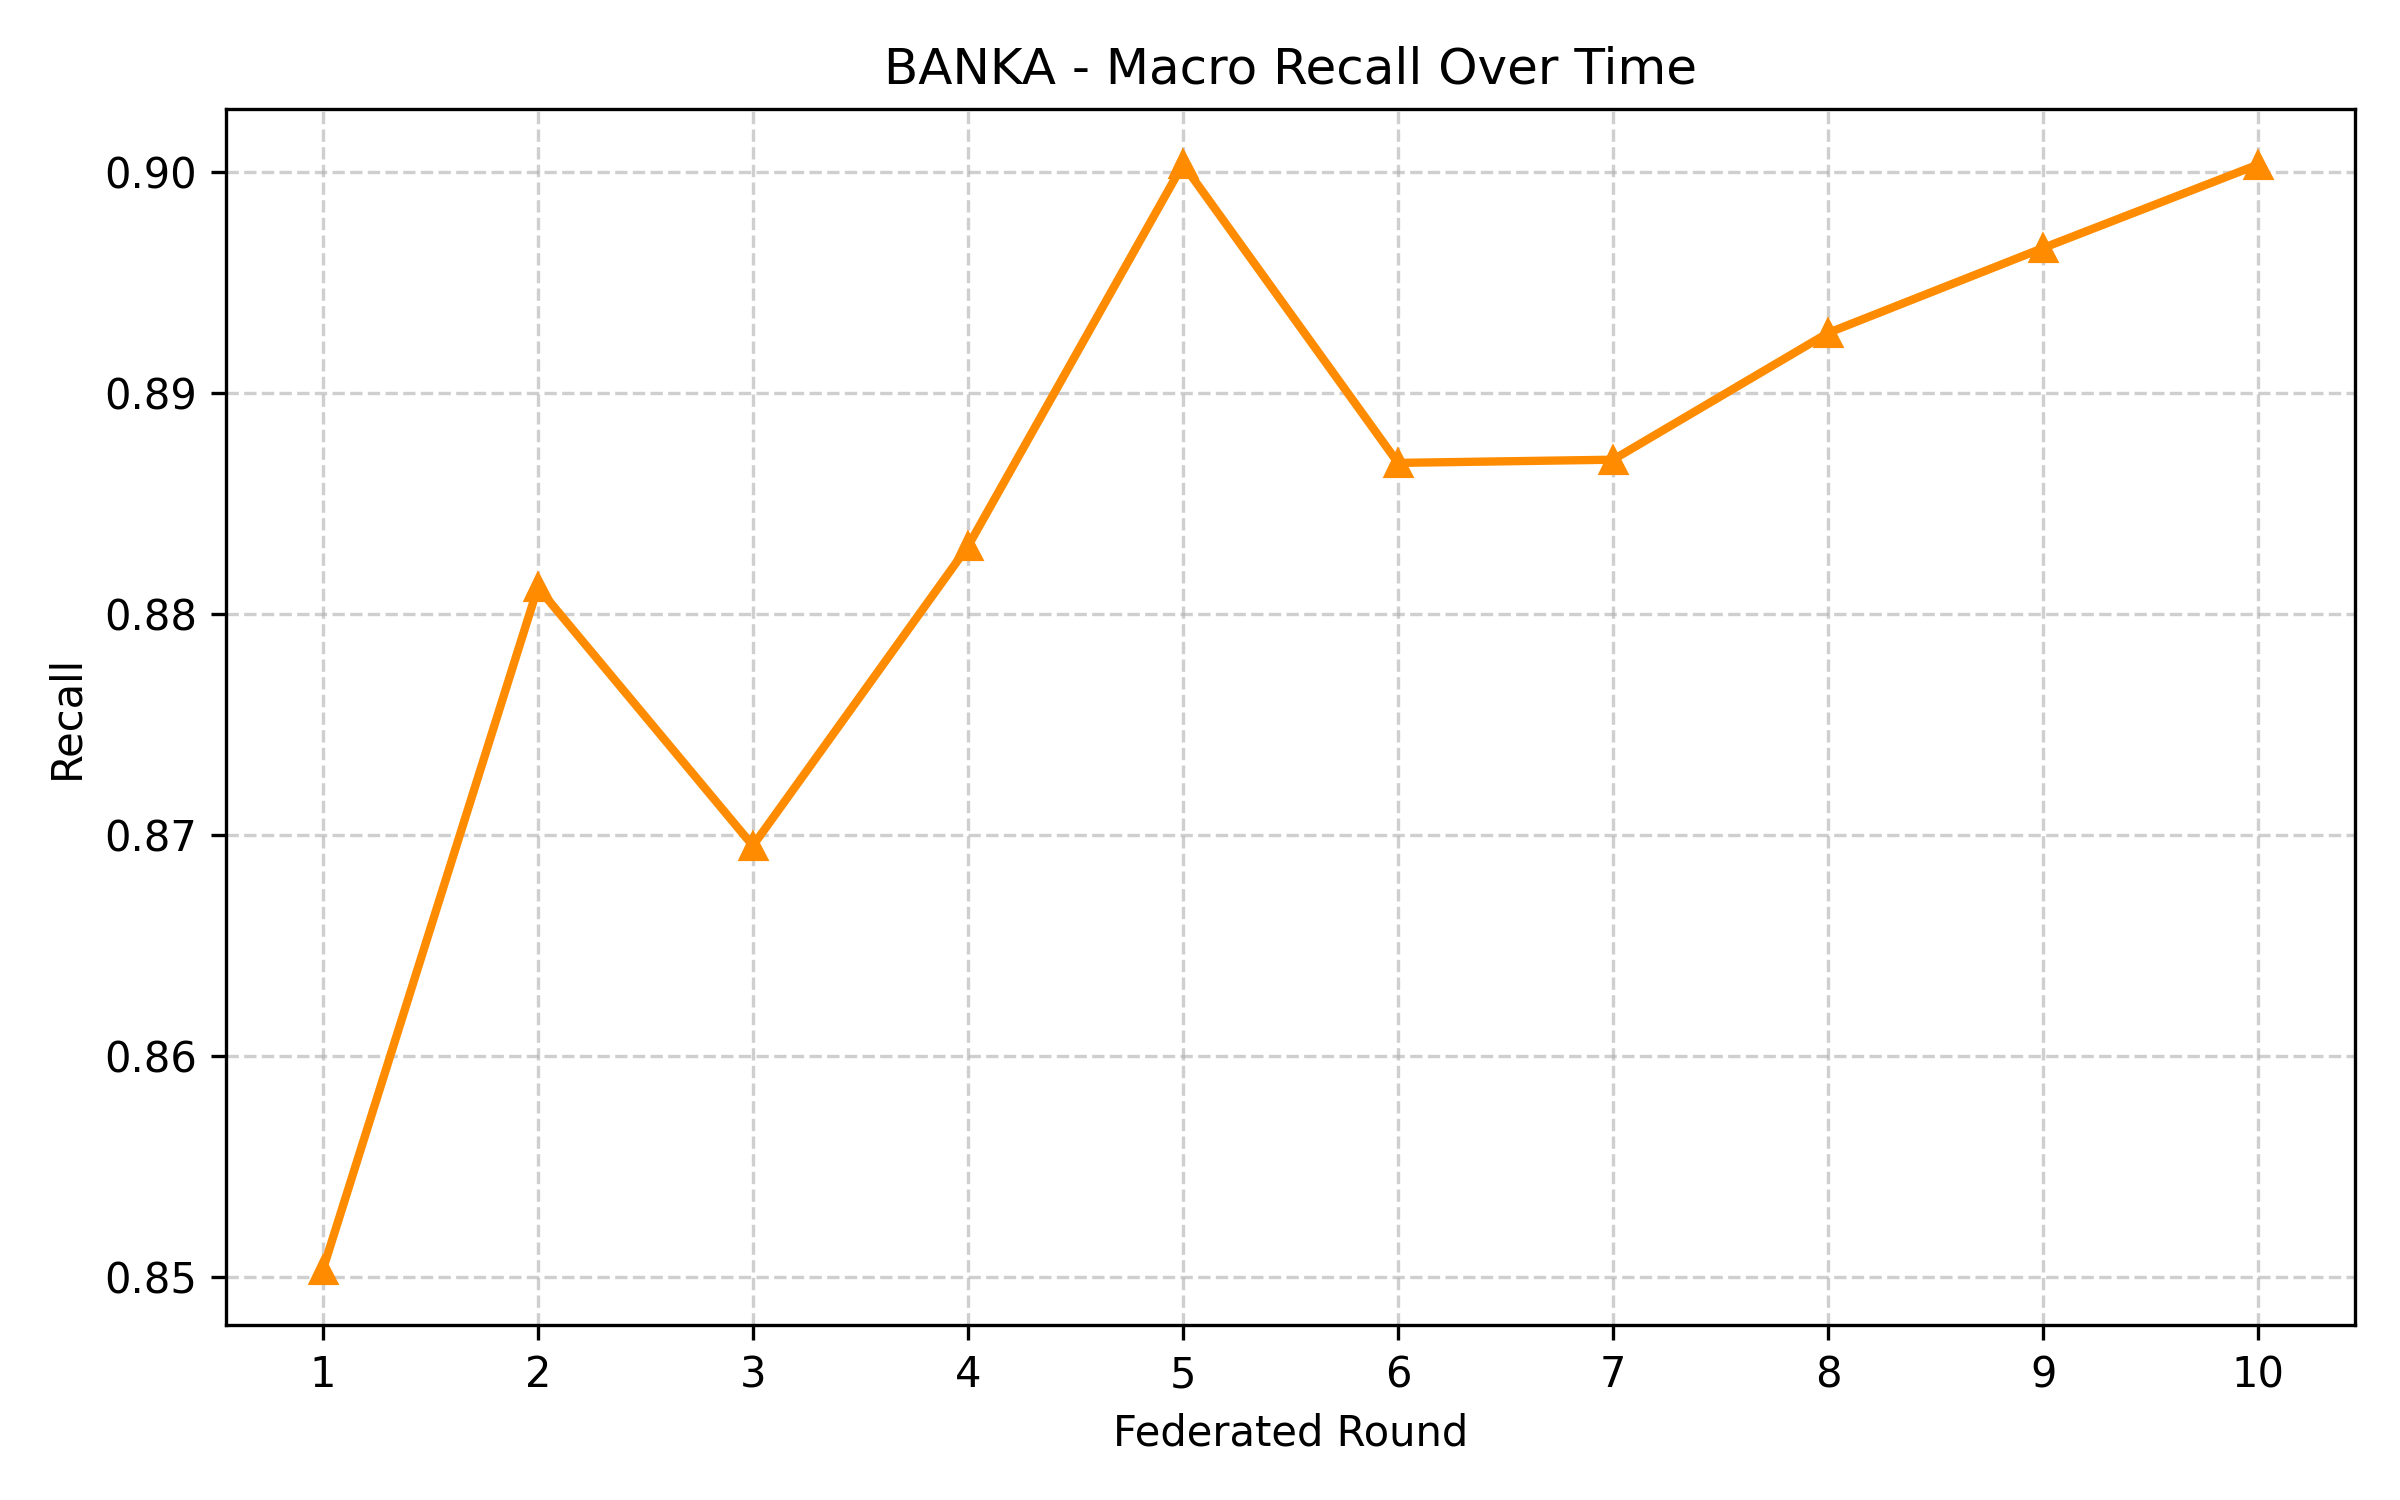
\includegraphics[width=\linewidth]{Figures/banka_progression_recall.png}

\vspace{0.1cm}
{\small (c) BANKA Recall vs Federated Aggregation Rounds}
\end{minipage}

\caption{BANKA Federated Accuracy, Precision, and Recall Progression Across Federated Aggregation Rounds}
\label{fig:banka_progression}
\end{figure}

The BANKA institutional client showed a steady increase in classification performance from round to round of federated aggregation as shown in Figure~\ref{fig:banka_progression}. The Accuracy, Precision and Recall values showed a general improvement with the going on of federated training, though minor changes were noted as it started. The accuracy rose steadily from 94.8\% to 96.5\%, and the Precision and Recall rose from 89.8\% to 91.5\% and 85.0\% to 90.0\%, respectively. The performance metrics showed less variance and more stability after the fifth aggregation round, suggesting successful convergence during the federated learning process. The observed evolution confirms the capability of distributed parameter aggregation to improve the generalization of the model and to ensure the same analytical performance in different institutional training context, without sharing any data at a central point.


%--------------------------------------------------------
\subsection{BANKB Federated Convergence}
%--------------------------------------------------------

\begin{figure}[H]
\centering

% Top Row
\begin{minipage}{0.48\textwidth}
\centering
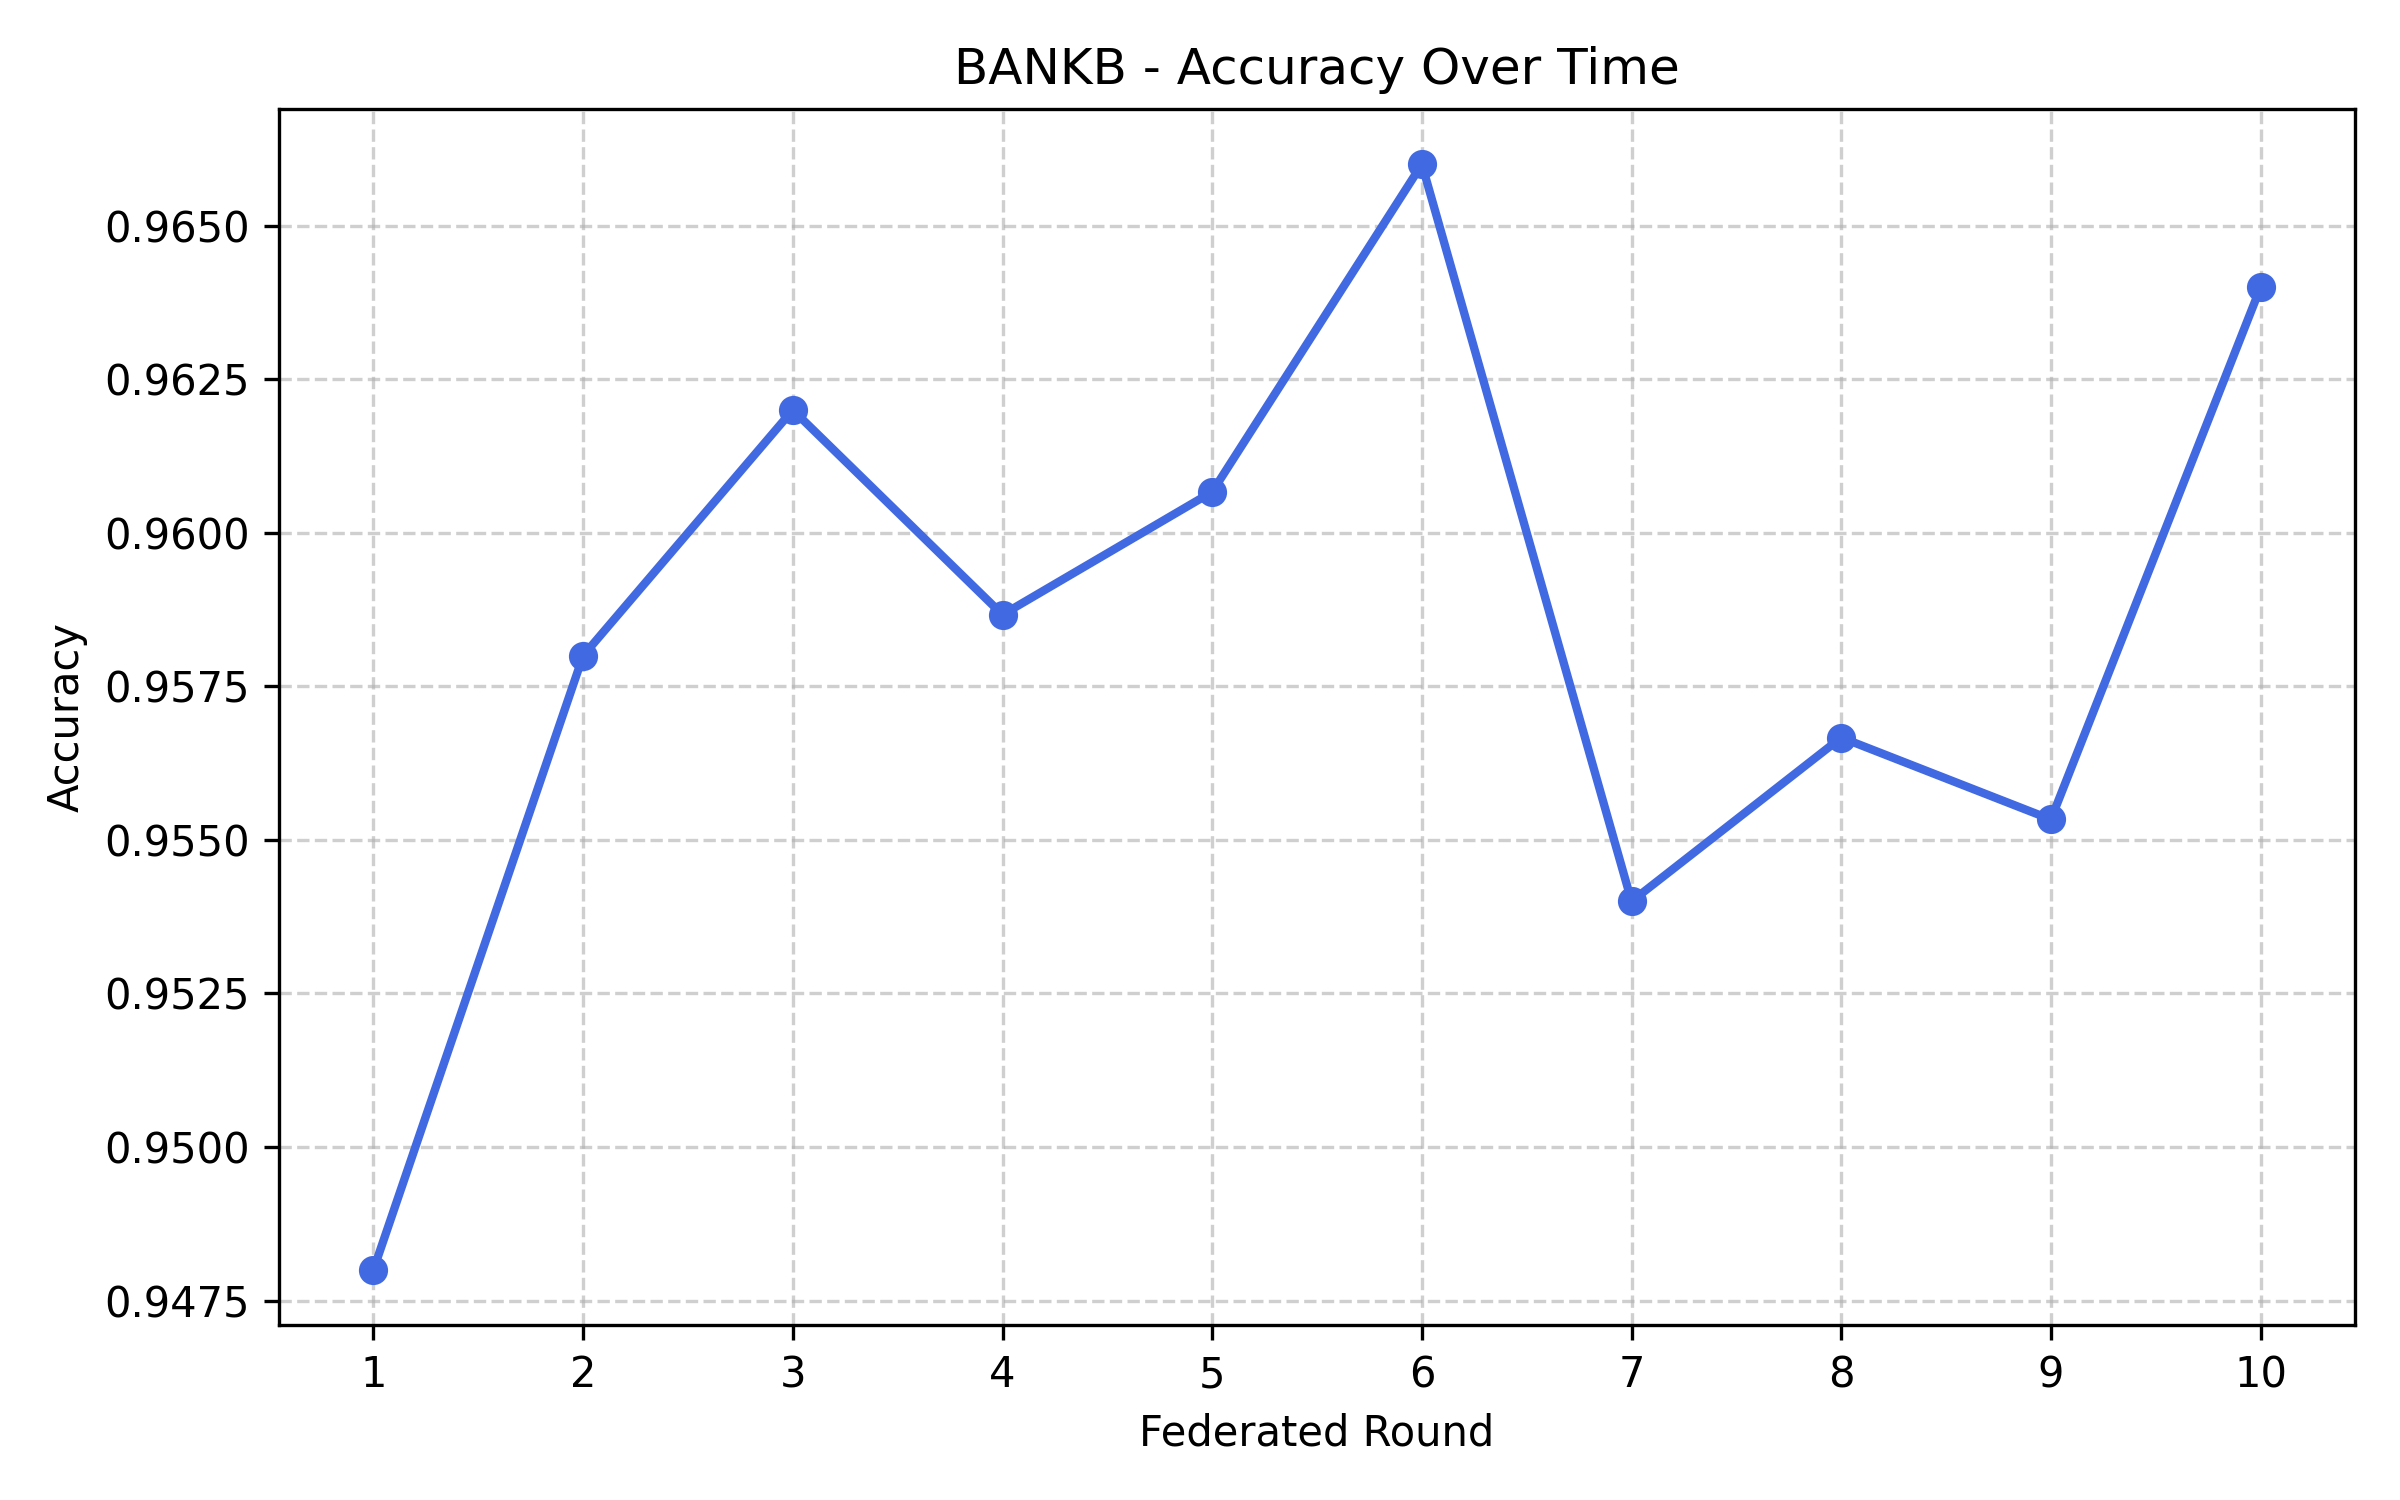
\includegraphics[width=\linewidth]{Figures/bankb_progression_accuracy.png}

\vspace{0.1cm}
{\small (a) BANKB Accuracy vs Federated Aggregation Rounds}
\end{minipage}
\hfill
\begin{minipage}{0.48\textwidth}
\centering
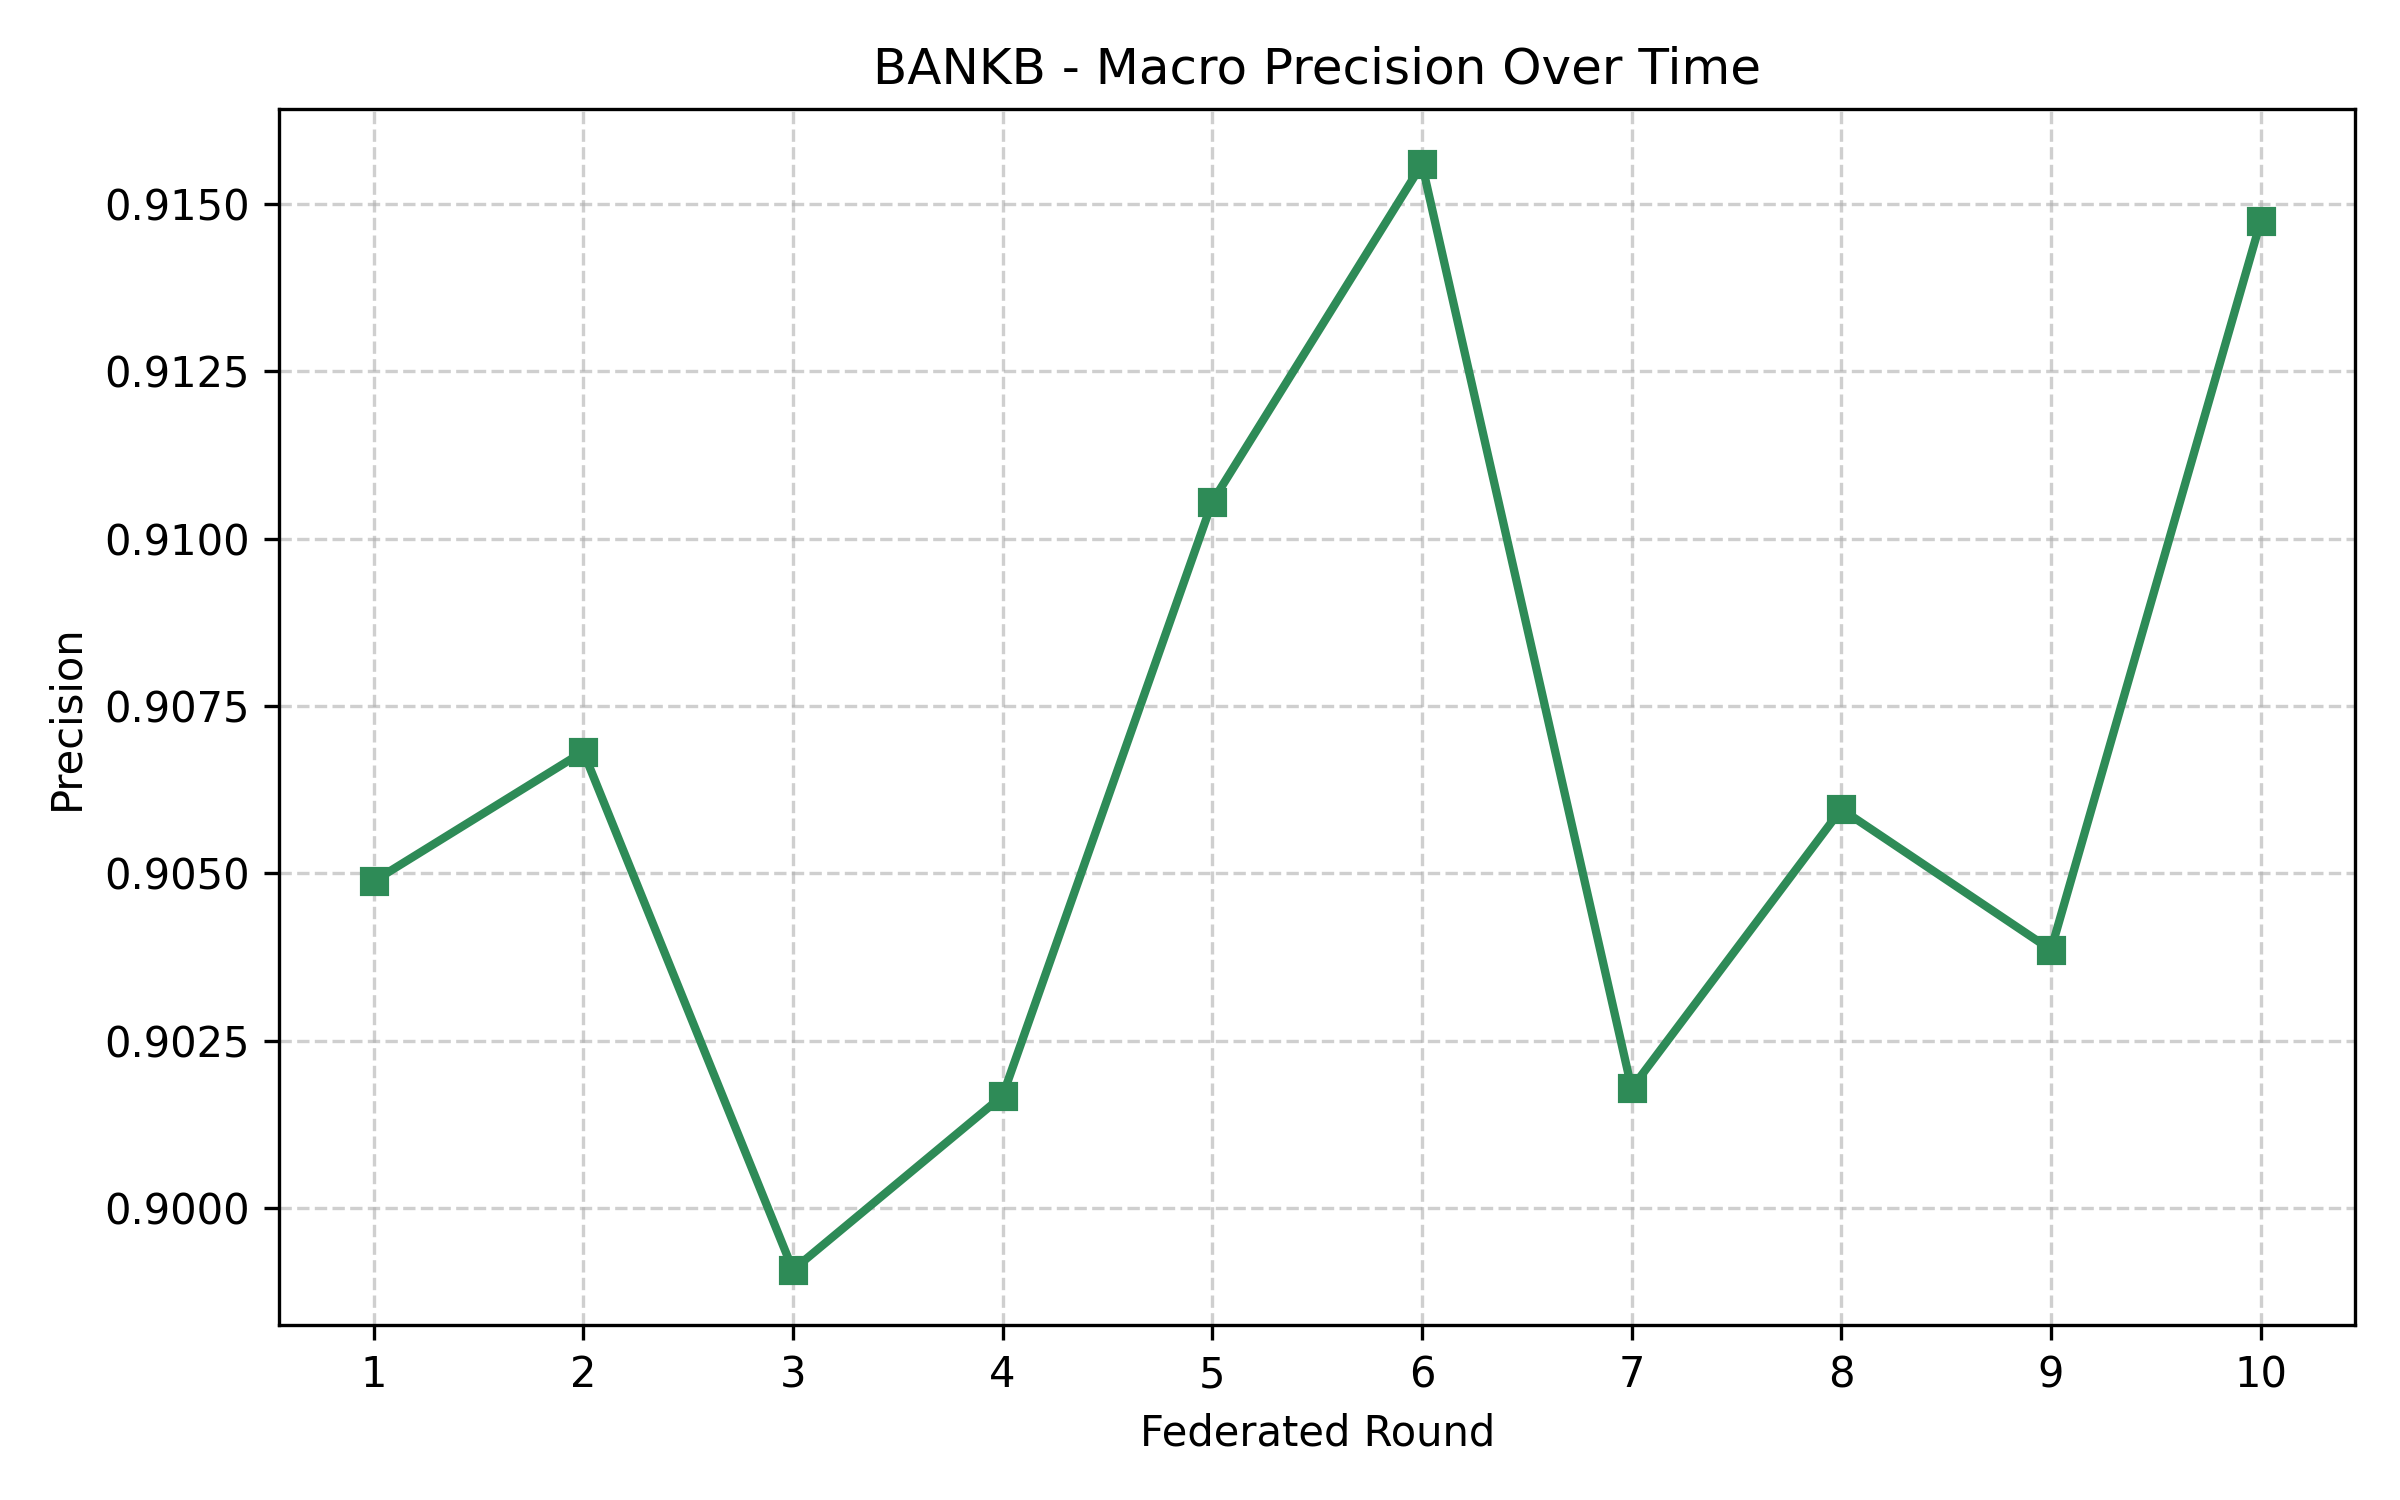
\includegraphics[width=\linewidth]{Figures/bankb_progression_precision.png}

\vspace{0.1cm}
{\small (b) BANKB Precision vs Federated Aggregation Rounds}
\end{minipage}

\vspace{0.4cm}

% Bottom Row
\begin{center}
\begin{minipage}{0.48\textwidth}
\centering
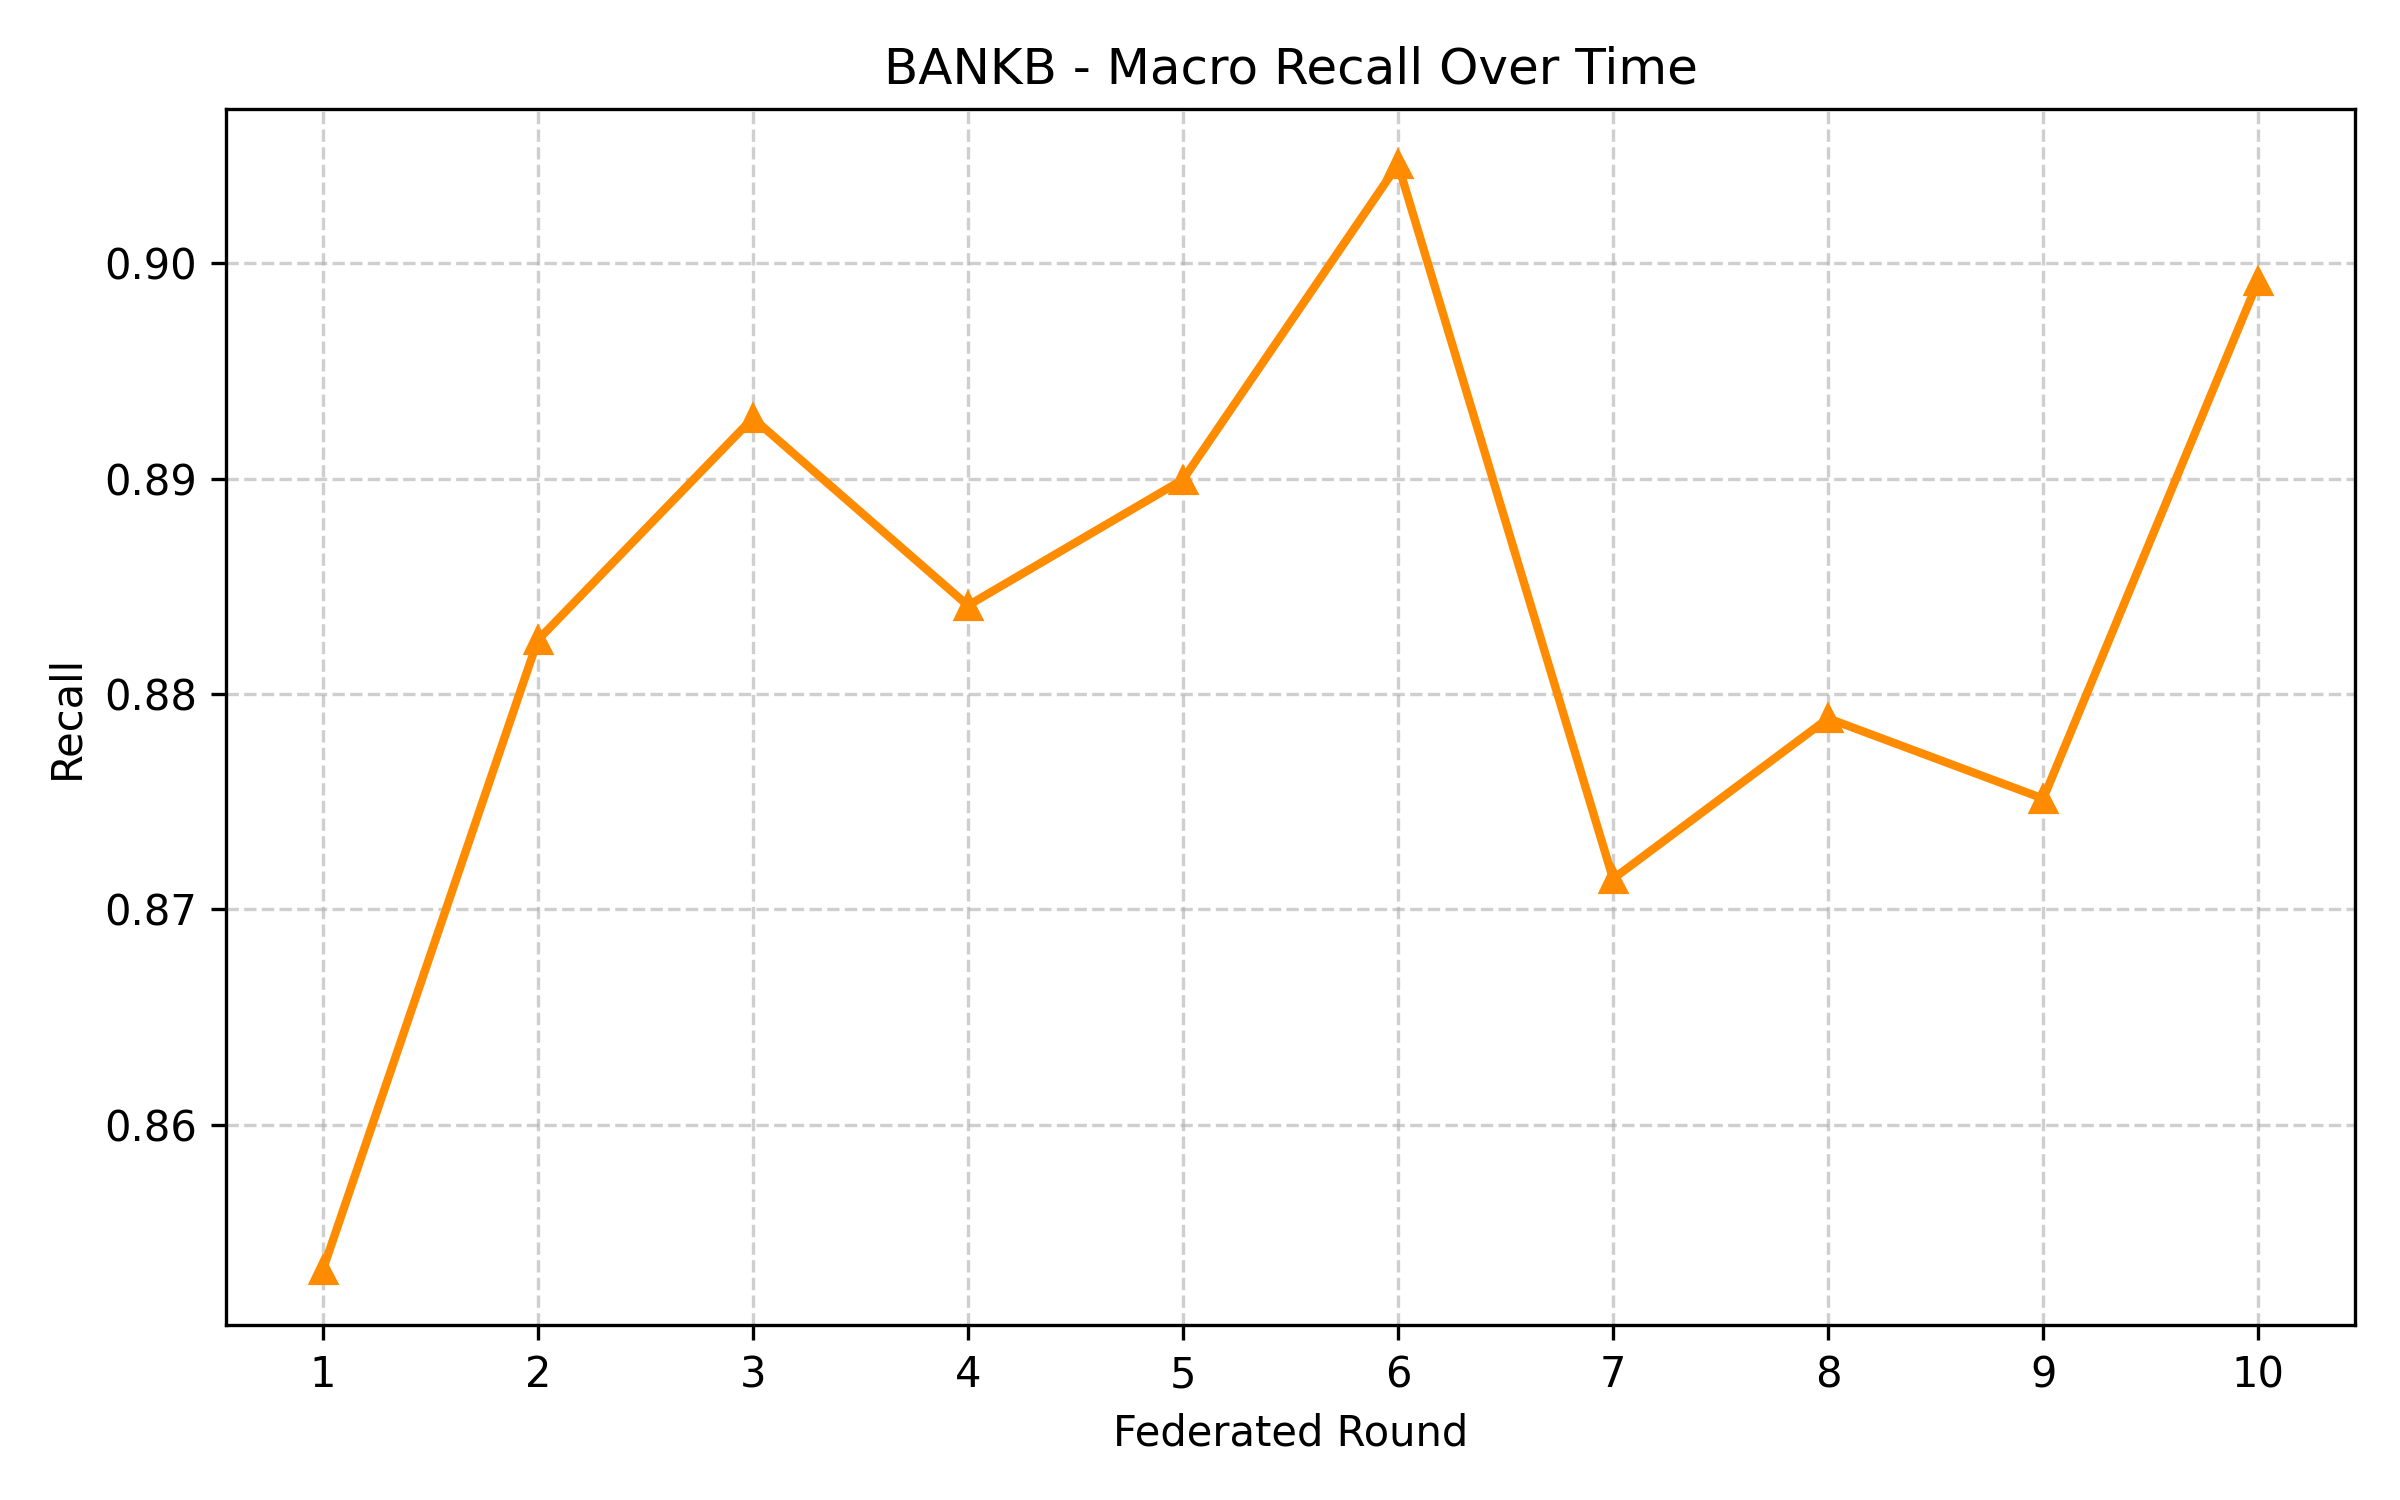
\includegraphics[width=\linewidth]{Figures/bankb_progression_recall.png}

\vspace{0.1cm}
{\small (c) BANKB Recall vs Federated Aggregation Rounds}
\end{minipage}
\end{center}

\caption{BANKB Federated Accuracy, Precision, and Recall Progression Across Federated Aggregation Rounds}
\label{fig:bankb_progression}
\end{figure}

he progressive improvement in classification performance of the BANKB institutional client can be seen in the successive rounds of federated aggregation (as shown in Figure~\ref{fig:bankb_progression}). Although there were some fluctuations in intermediate communication rounds, there was an overall increase in Accuracy, Precision, and Recall. The accuracy rose from ~94.8\% to 96.4\%, while Precision and Recall were improved from 90.5\% to 91.5\%, 85.3\% to 89.9\%, respectively. Stable parameter synchronization and subsequent updates were demonstrated as additional federated updates were applied to recover temporary performance fluctuations seen in later rounds of the experiment.Stable parameter synchronization and further model development was evidenced by additional federated updates in subsequent rounds of the experiment, which recovered temporary performance variations observed in earlier rounds. The final aggregation rounds delivered very robust analytical results with a level of federated convergence and knowledge sharing between distributed institutional training environments that did not provide any centralised data exchange.

%--------------------------------------------------------
\subsection{BANKC Federated Convergence}
%--------------------------------------------------------
\begin{figure}[H]
\centering

% Top Row
\begin{minipage}{0.48\textwidth}
\centering
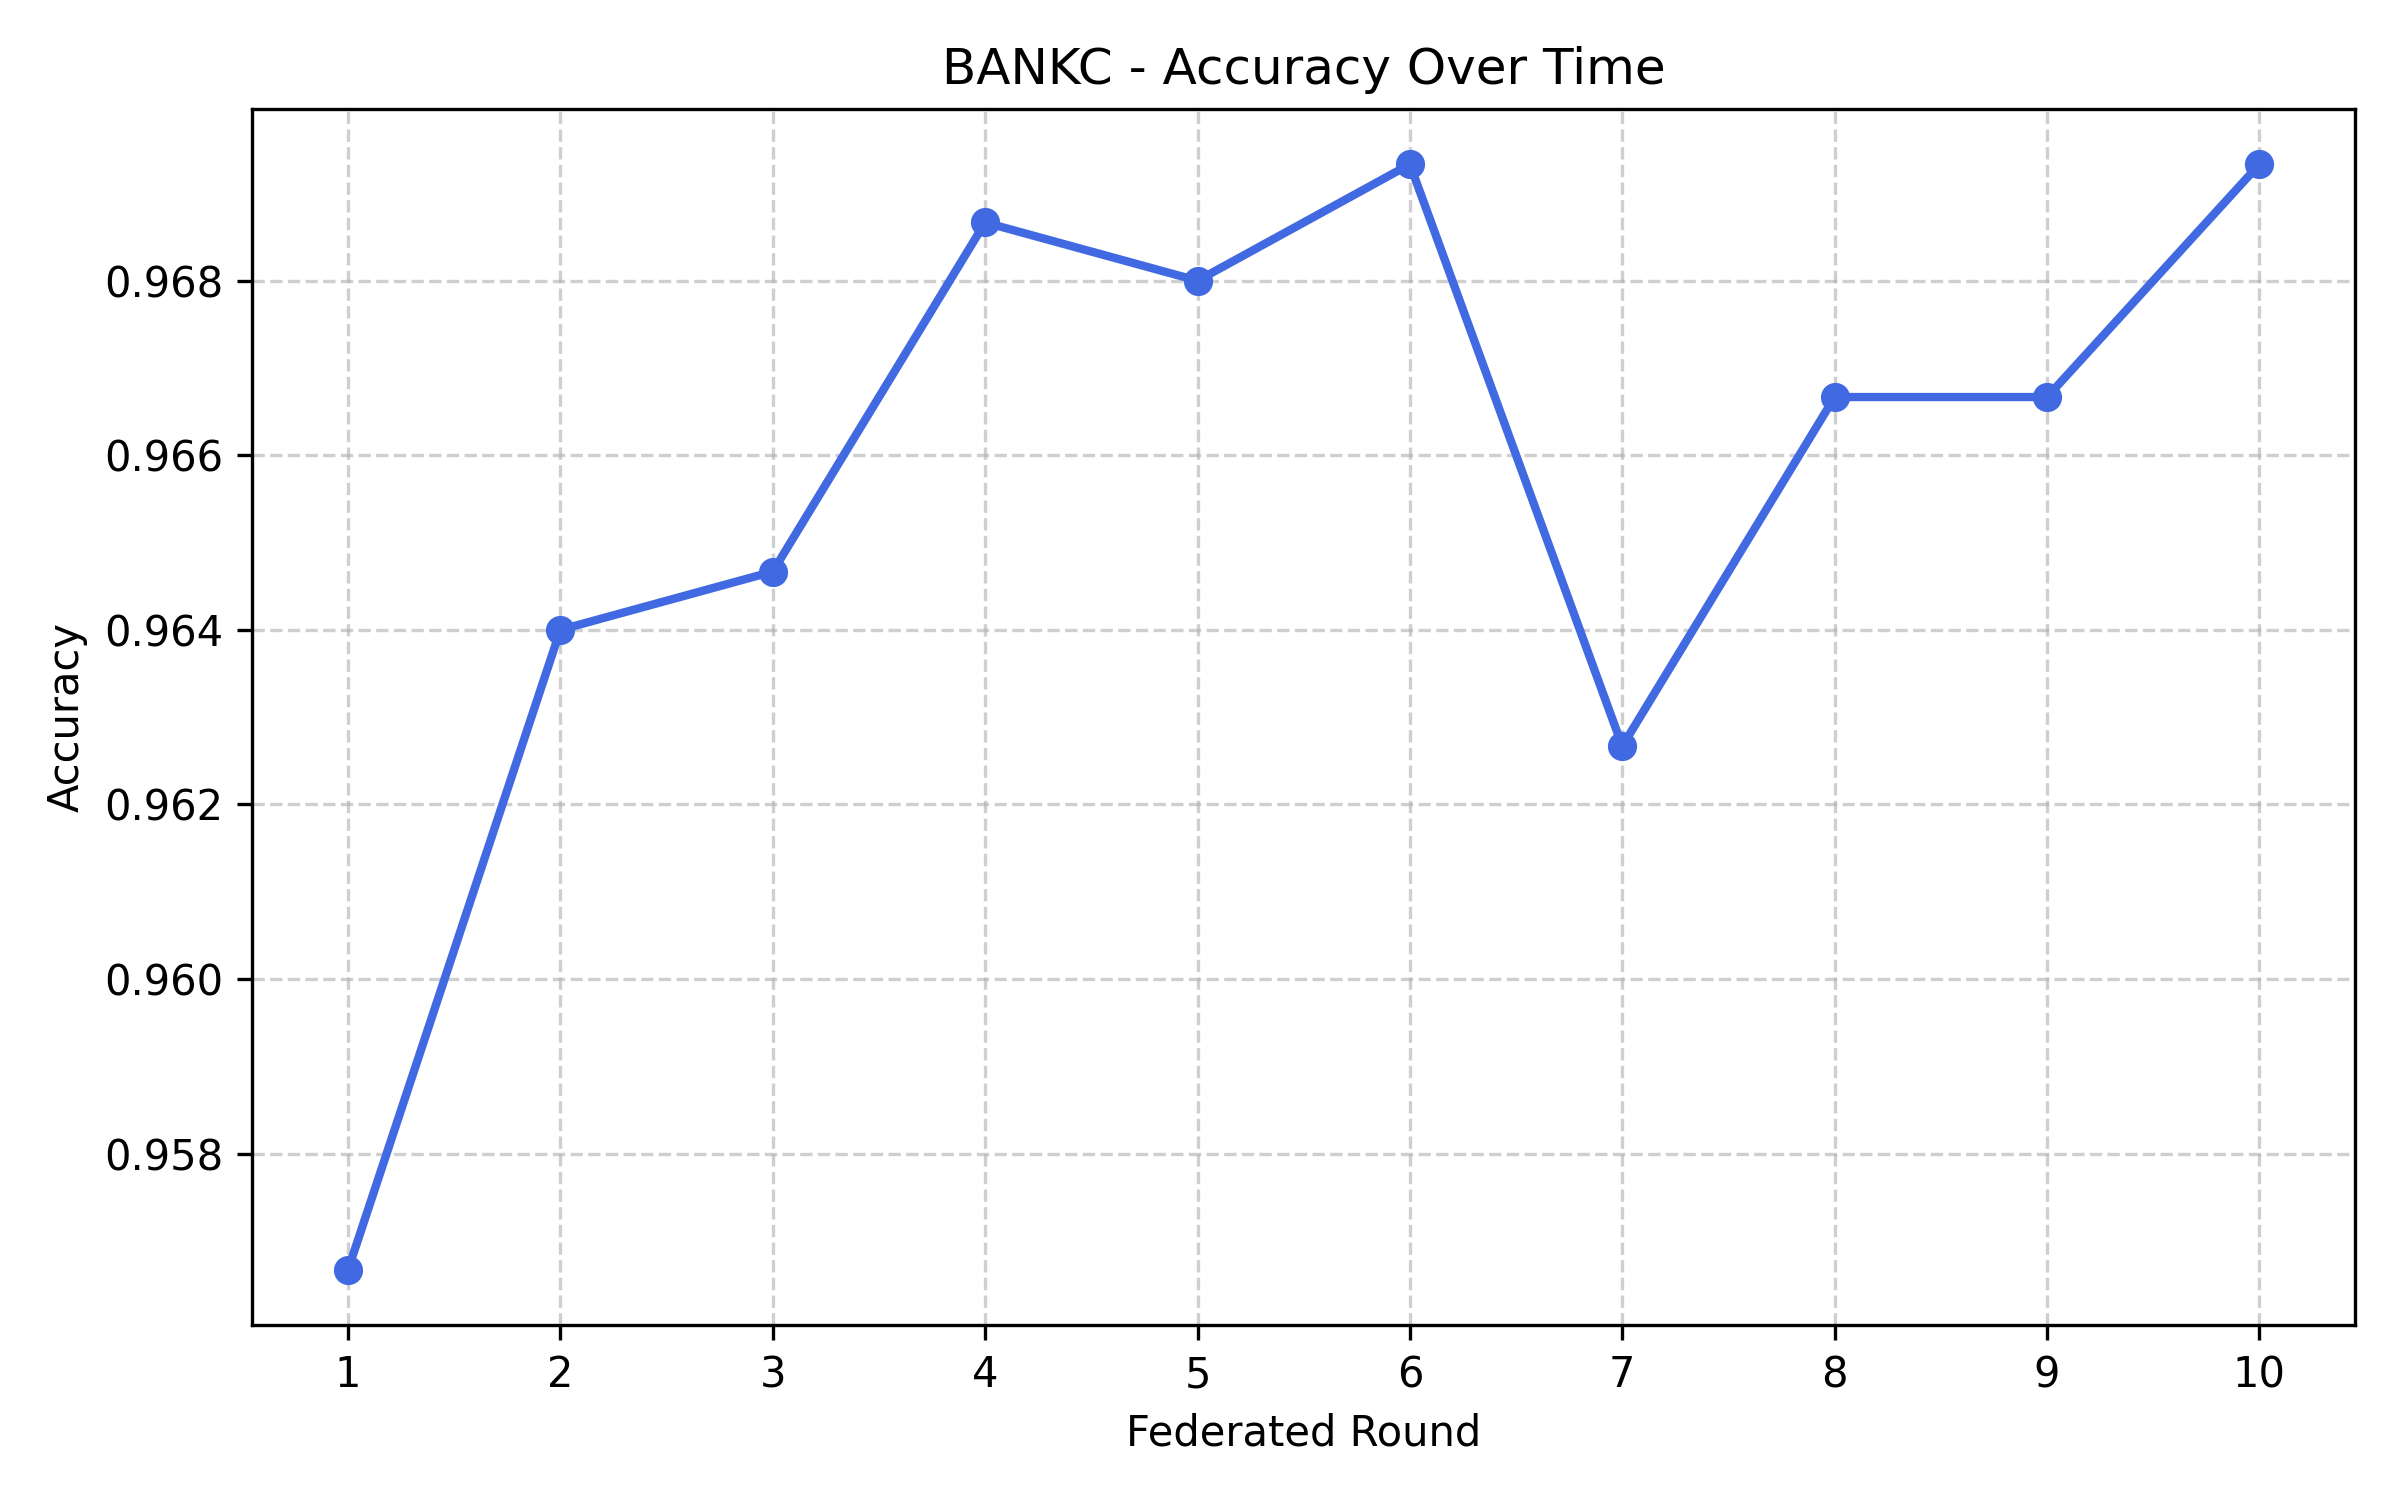
\includegraphics[width=\linewidth]{Figures/bankc_progression_accuracy.png}

\vspace{0.1cm}
{\small (a) BANKC Accuracy vs Federated Aggregation Rounds}
\end{minipage}
\hfill
\begin{minipage}{0.48\textwidth}
\centering
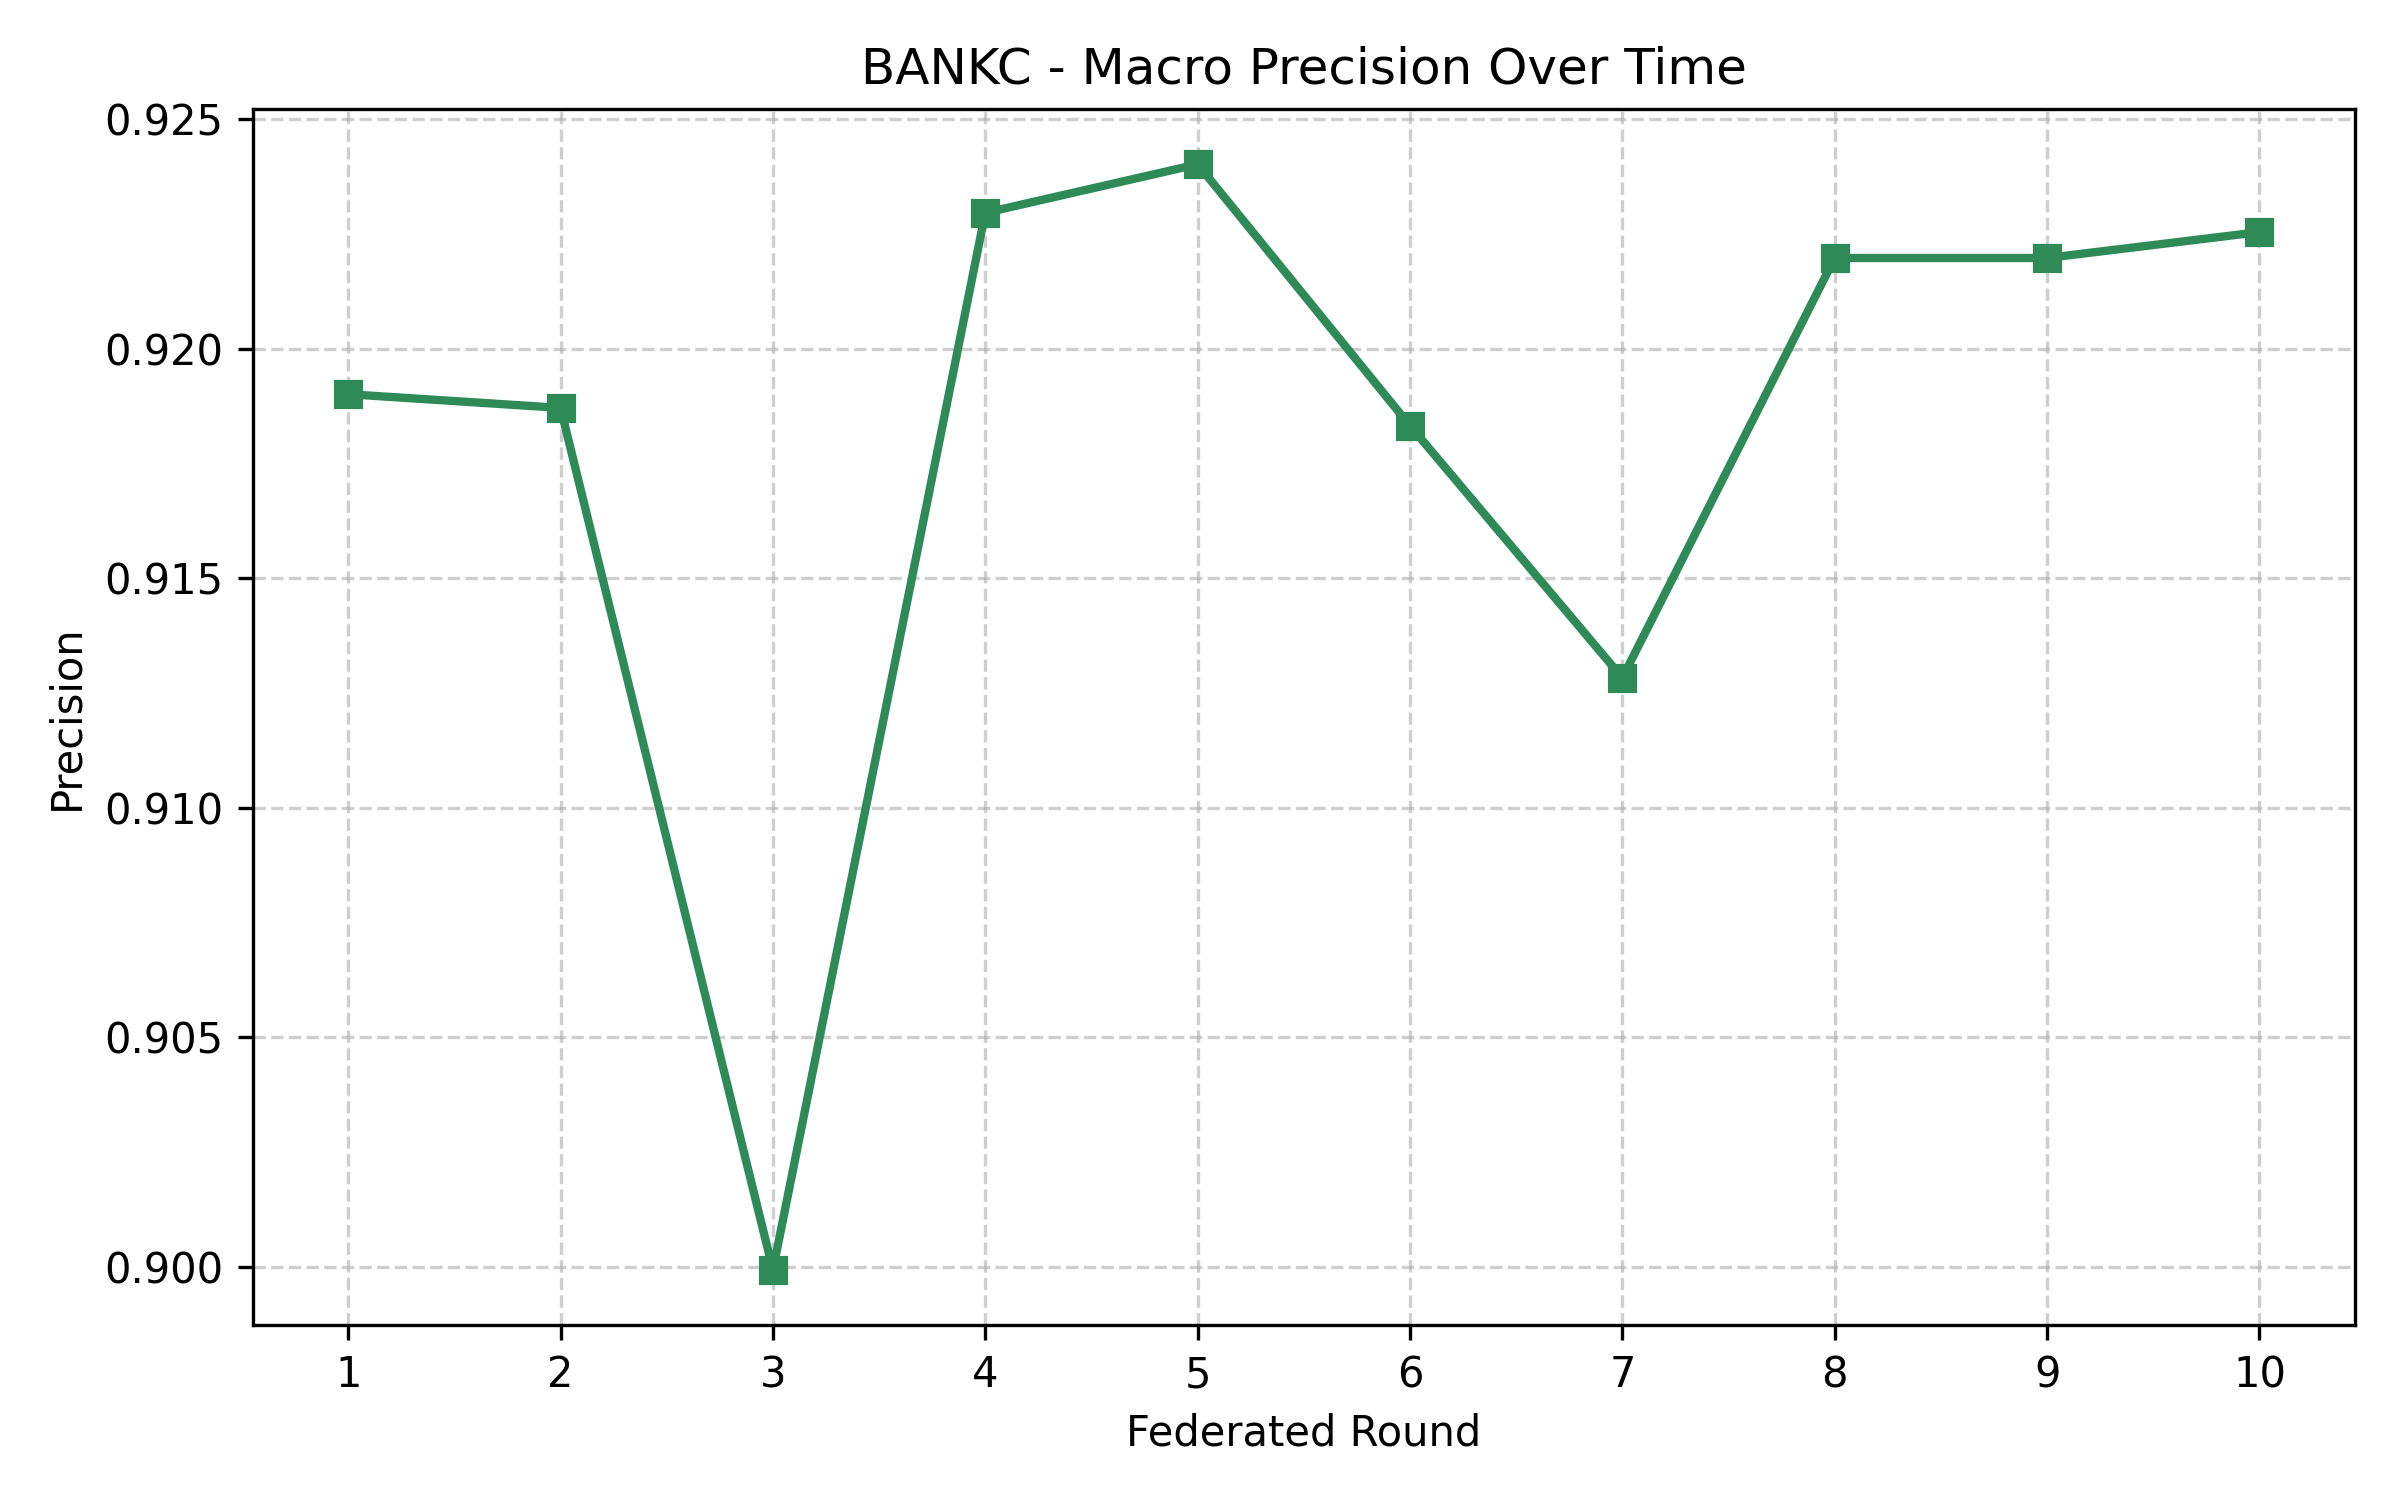
\includegraphics[width=\linewidth]{Figures/bankc_progression_precision.png}

\vspace{0.1cm}
{\small (b) BANKC Precision vs Federated Aggregation Rounds}
\end{minipage}

\vspace{0.4cm}

% Bottom Row
\begin{center}
\begin{minipage}{0.48\textwidth}
\centering
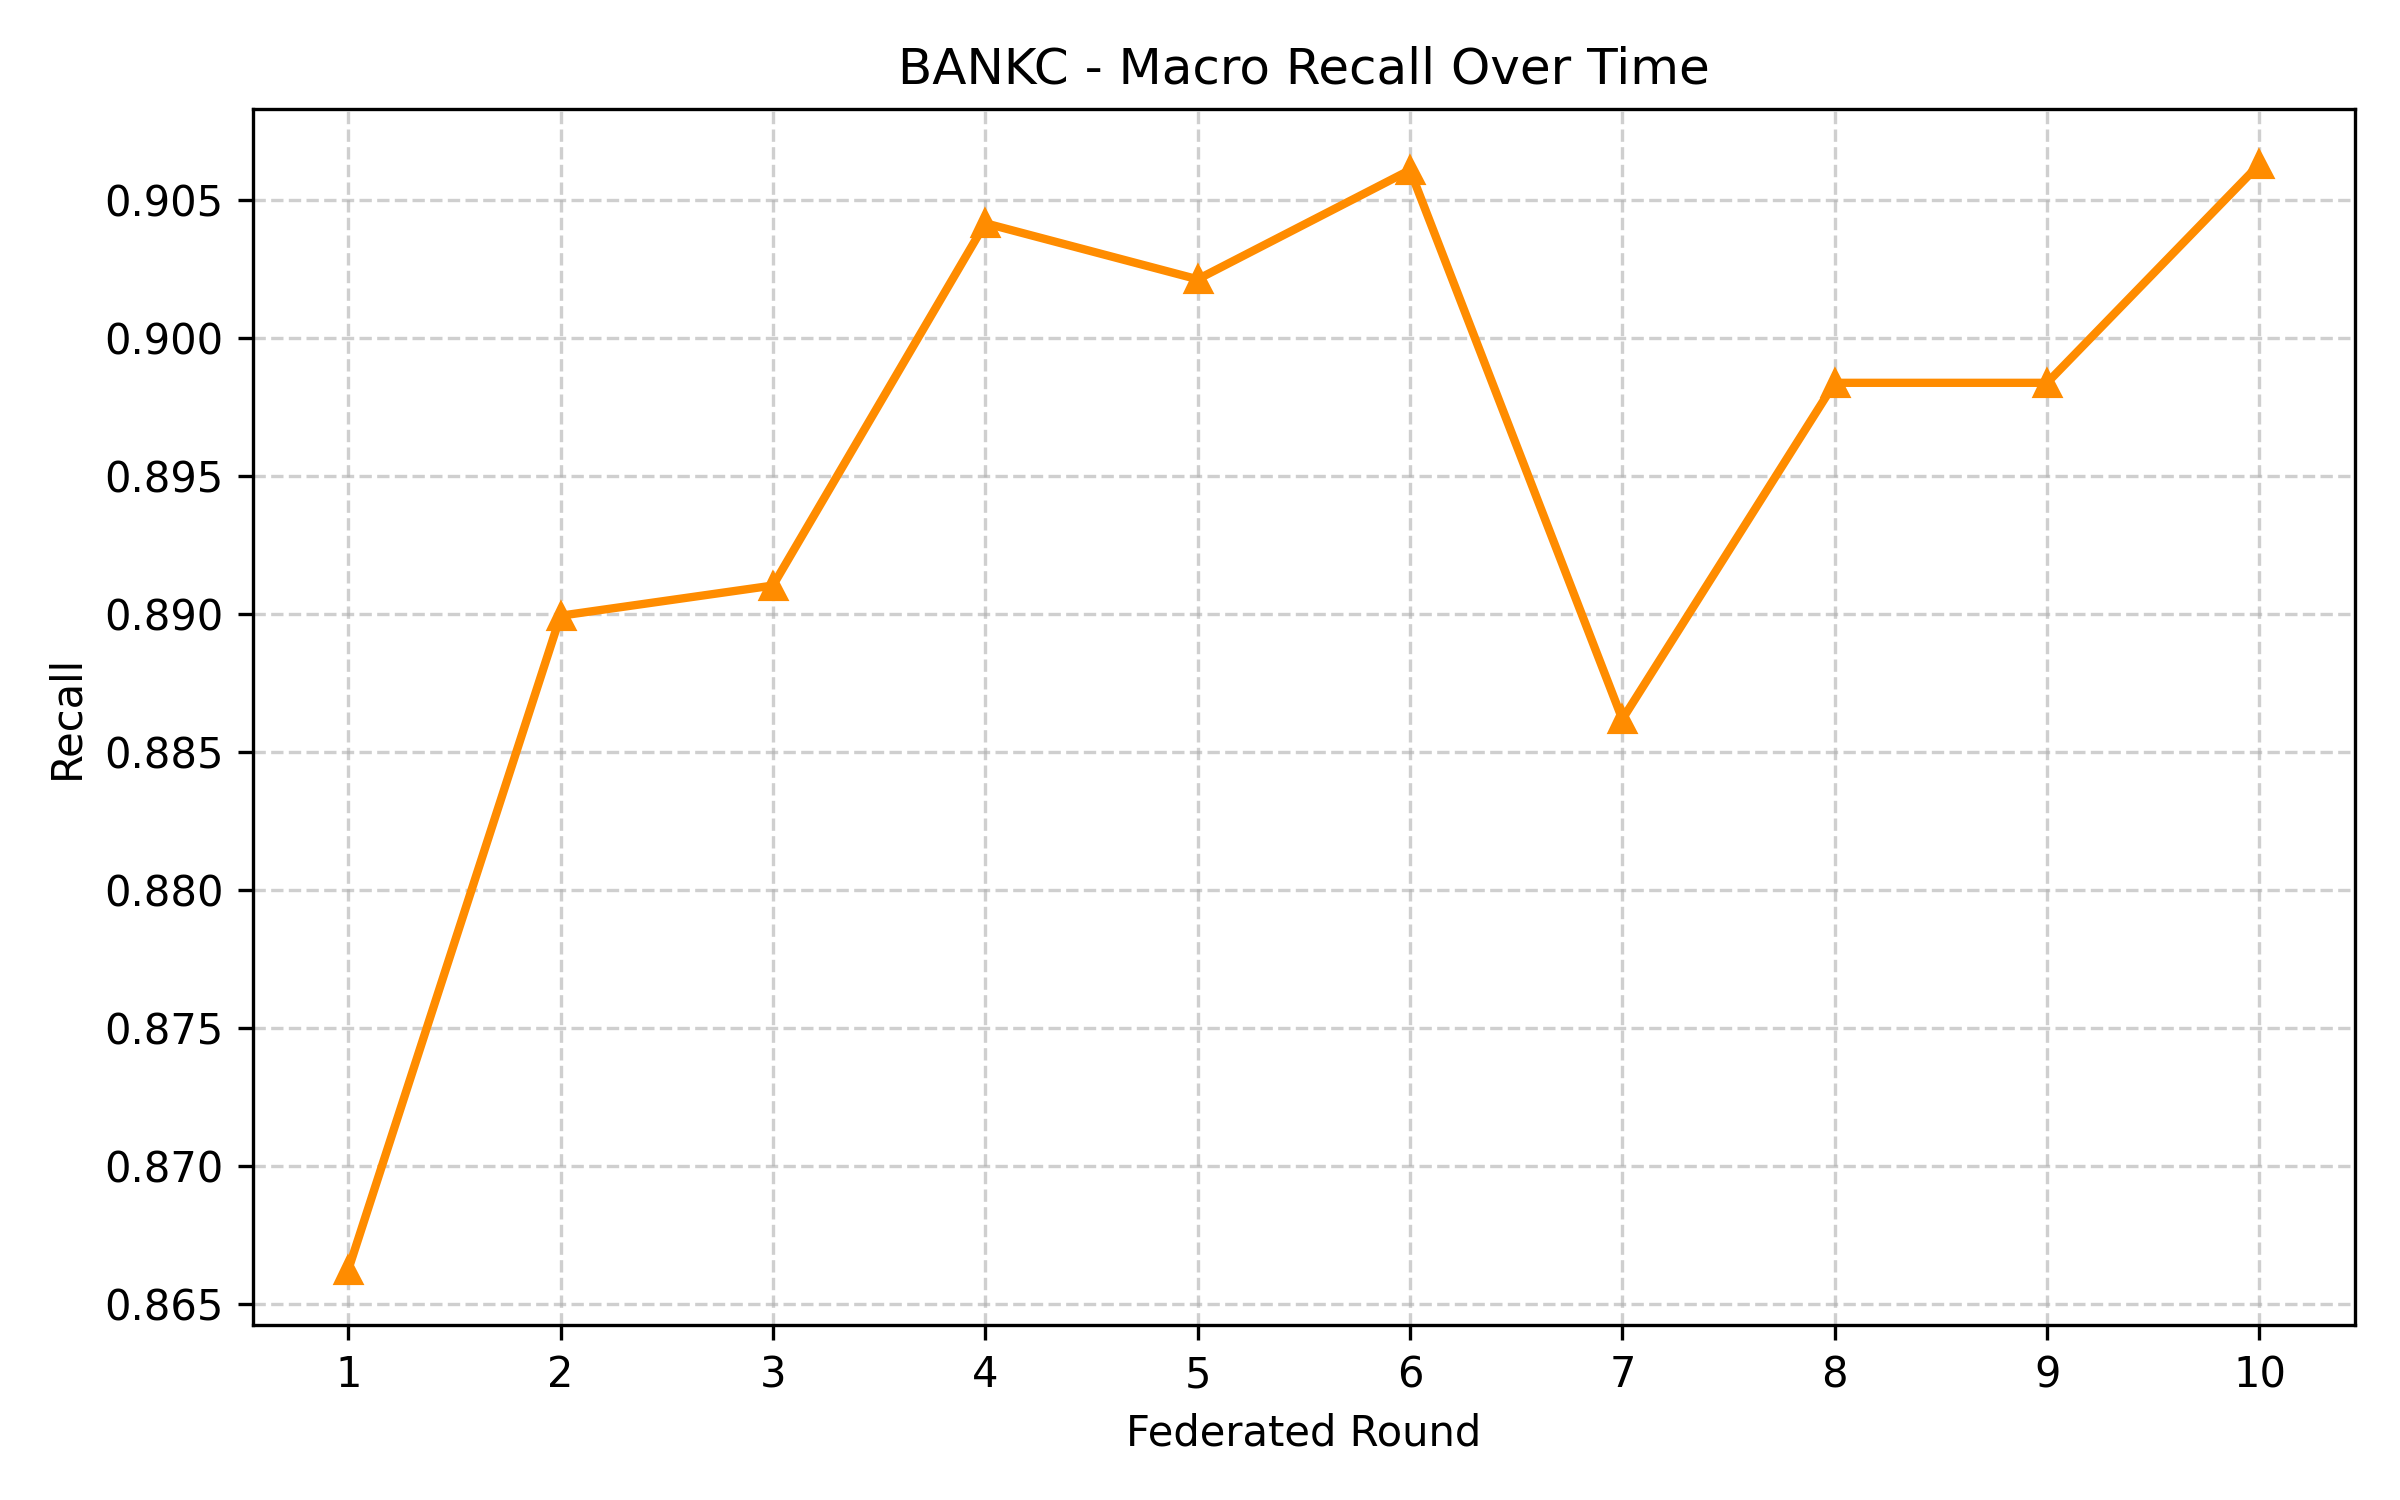
\includegraphics[width=\linewidth]{Figures/bankc_progression_recall.png}

\vspace{0.1cm}
{\small (c) BANKC Recall vs Federated Aggregation Rounds}
\end{minipage}
\end{center}

\caption{BANKC Federated Accuracy, Precision, and Recall Progression Across Federated Aggregation Rounds}
\label{fig:bankc_progression}
\end{figure}
The BANKC institutional client showed a very consistent federated convergence behaviour for successive aggregation rounds as shown in Figure~\ref{fig:bankc_progression}. The metrics of Accuracy (ACC), Precision (PRC), and Recall (RCL) all showed a gradual increase in the first few rounds of the initial communication phase, but afterwards, the data for the rest of the federated rounds were relatively stable with only slight variations. The accuracy elevates from about 95.7% to 96.9%, Precision and Recall reaches almost 92.2% and 90.6% respectively. Minimal performance fluctuations were noted at intermediate synchronization phases, although the metrics quickly stabilized and stayed in a small range, suggesting the successful distributed parameter aggregation and good model generalization. The observed convergence characteristics confirm the stable federated optimization and the framework's capability to keep the analytical performance stable in a heterogeneous institutional transaction environment while keeping the data out of the central repository.
%========================================================
\subsection[Precision--Recall and Confusion Matrix Validation]{\textbf{Precision--Recall and Confusion Matrix Validation}}
%========================================================

Precision-Recall analytical validation and confusion matrix analysis was performed to test for discrimination capabilities against fraud, minority class recognition behavior, and false positive propagation within distributed institutional settings. As fraudulent transactional activity accounted for only a small percentage of all transactional activity within institutions, Precision-Recall validation offered a more practical test than pure classification accuracy.
BANKA Precision-Recall and Confusion Matrix Validation


%--------------------------------------------------------
\subsubsection{BANKA Precision--Recall and Confusion Matrix Validation}
%--------------------------------------------------------

\begin{figure}[H]
\centering

\begin{minipage}{0.48\textwidth}
\centering
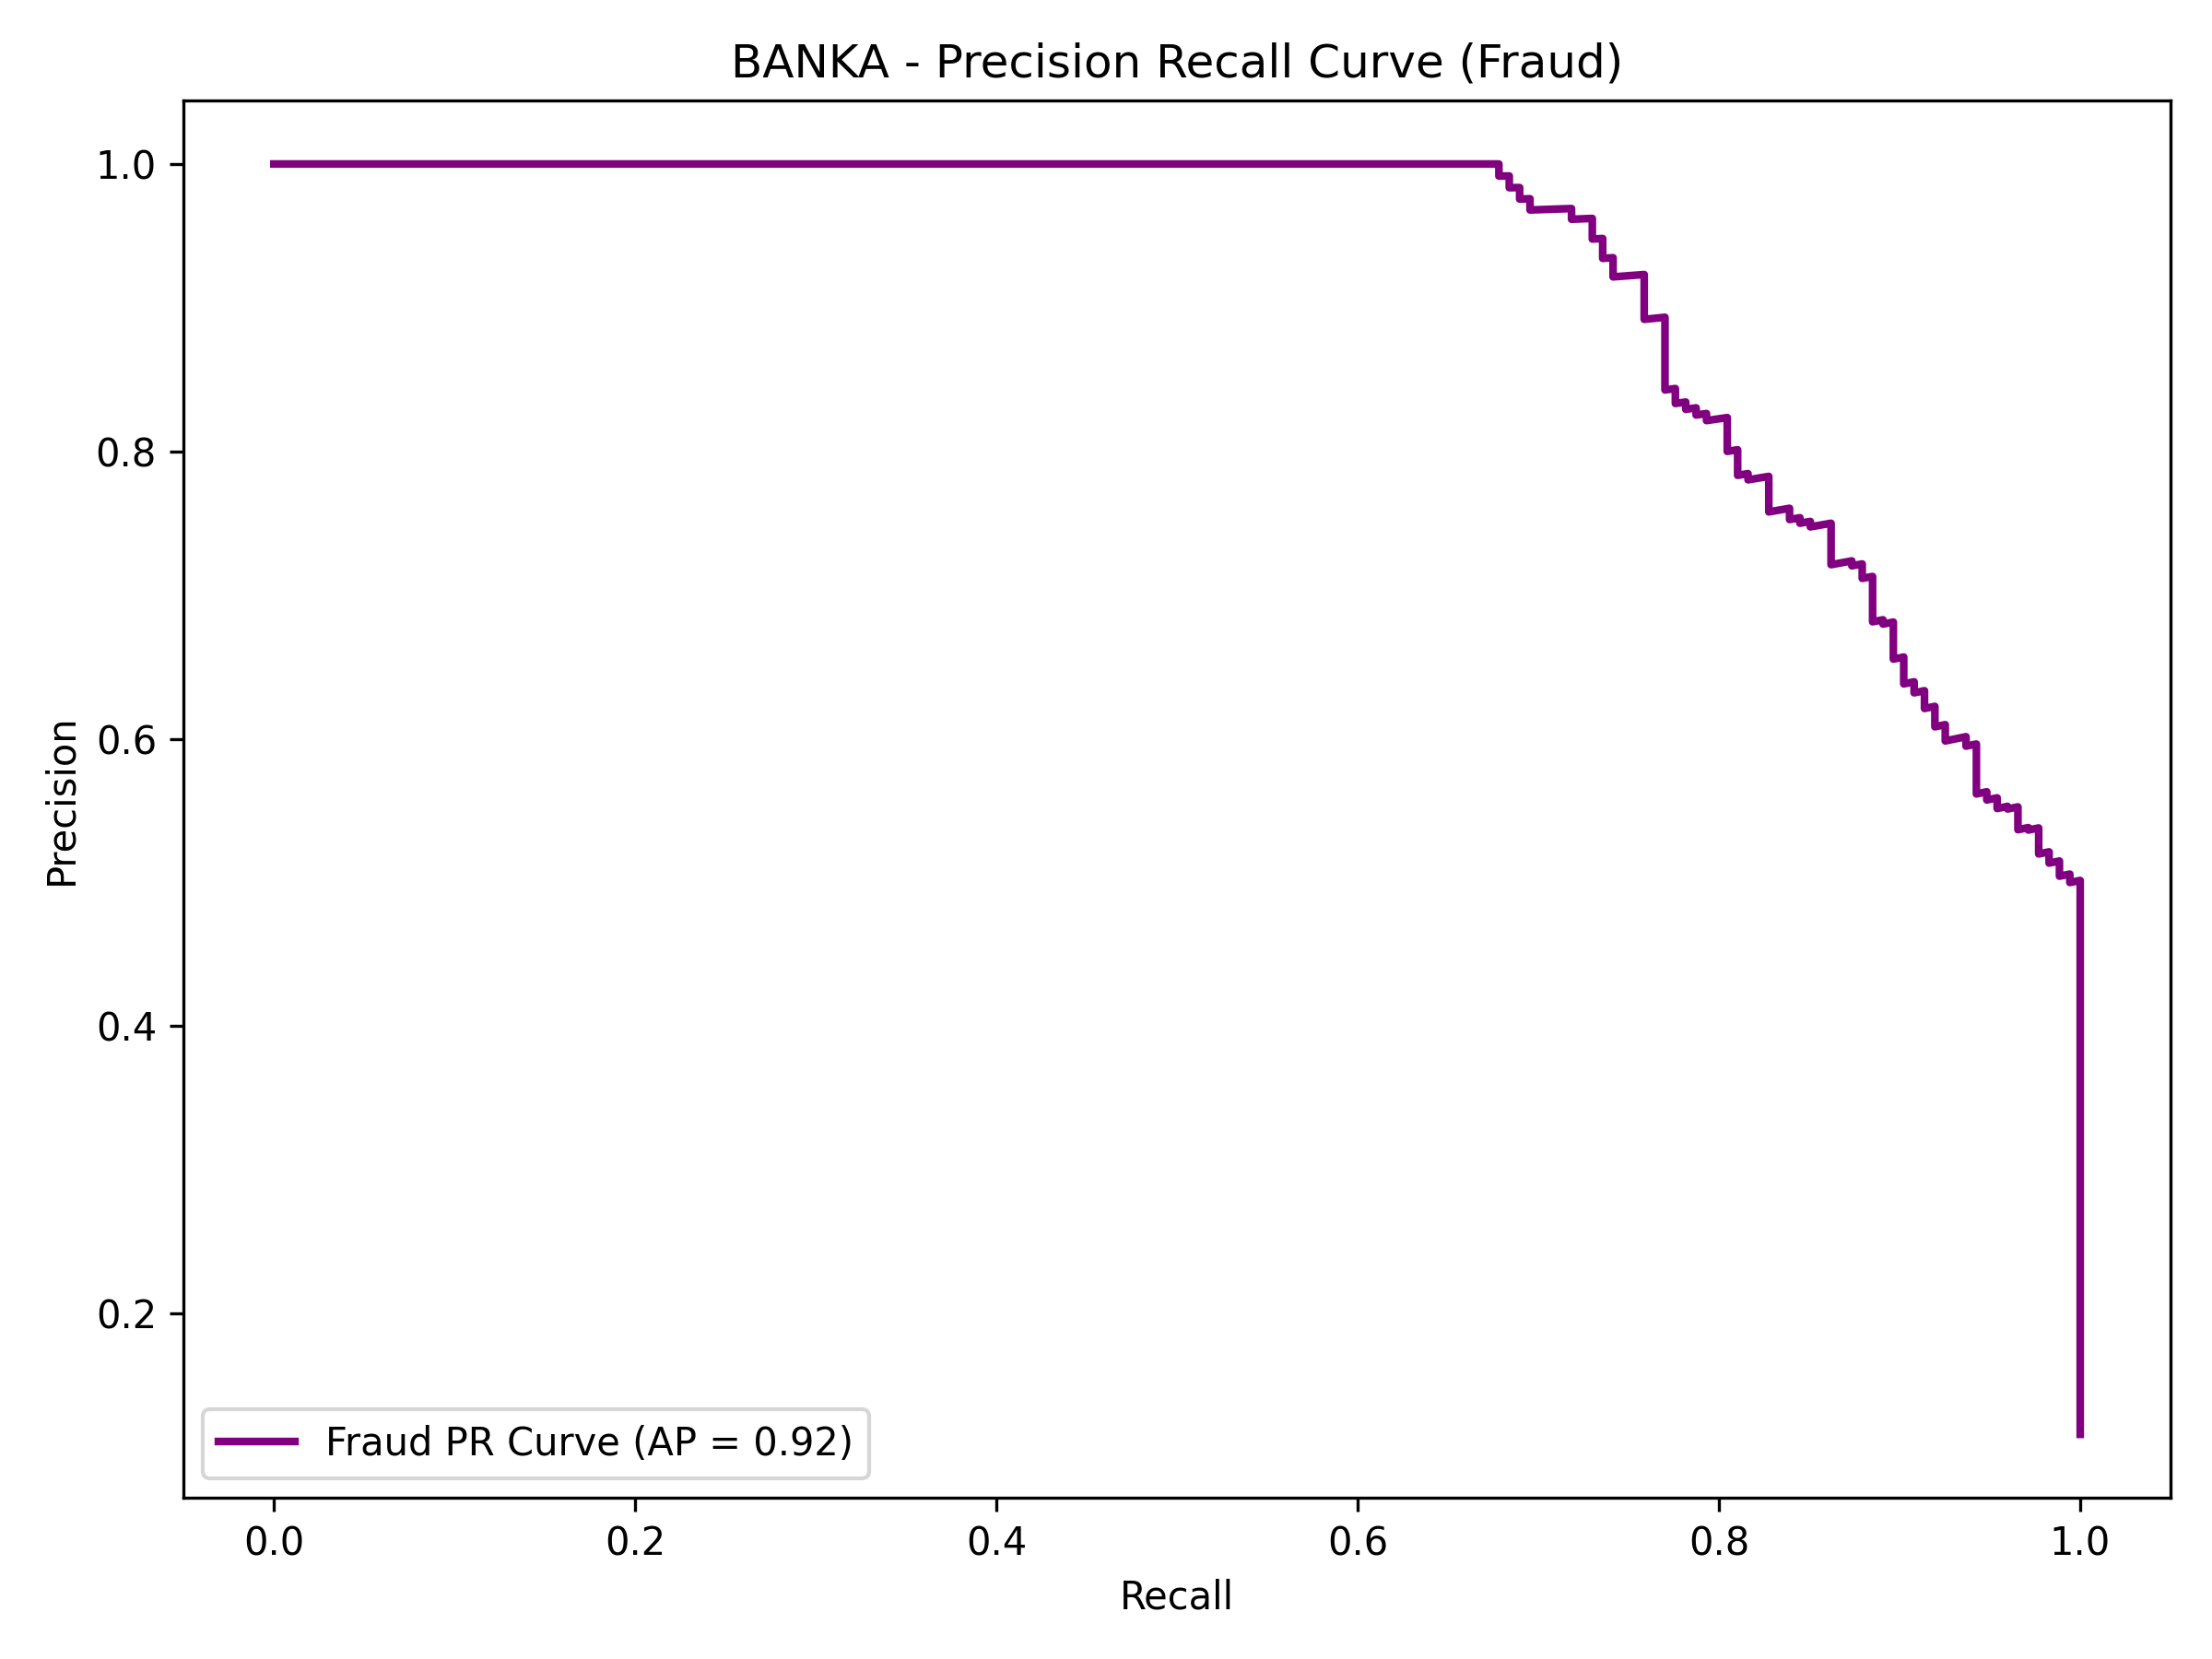
\includegraphics[width=\linewidth]{Figures/banka_pr_curve_deep.png}
\end{minipage}
\hfill
\begin{minipage}{0.48\textwidth}
\centering
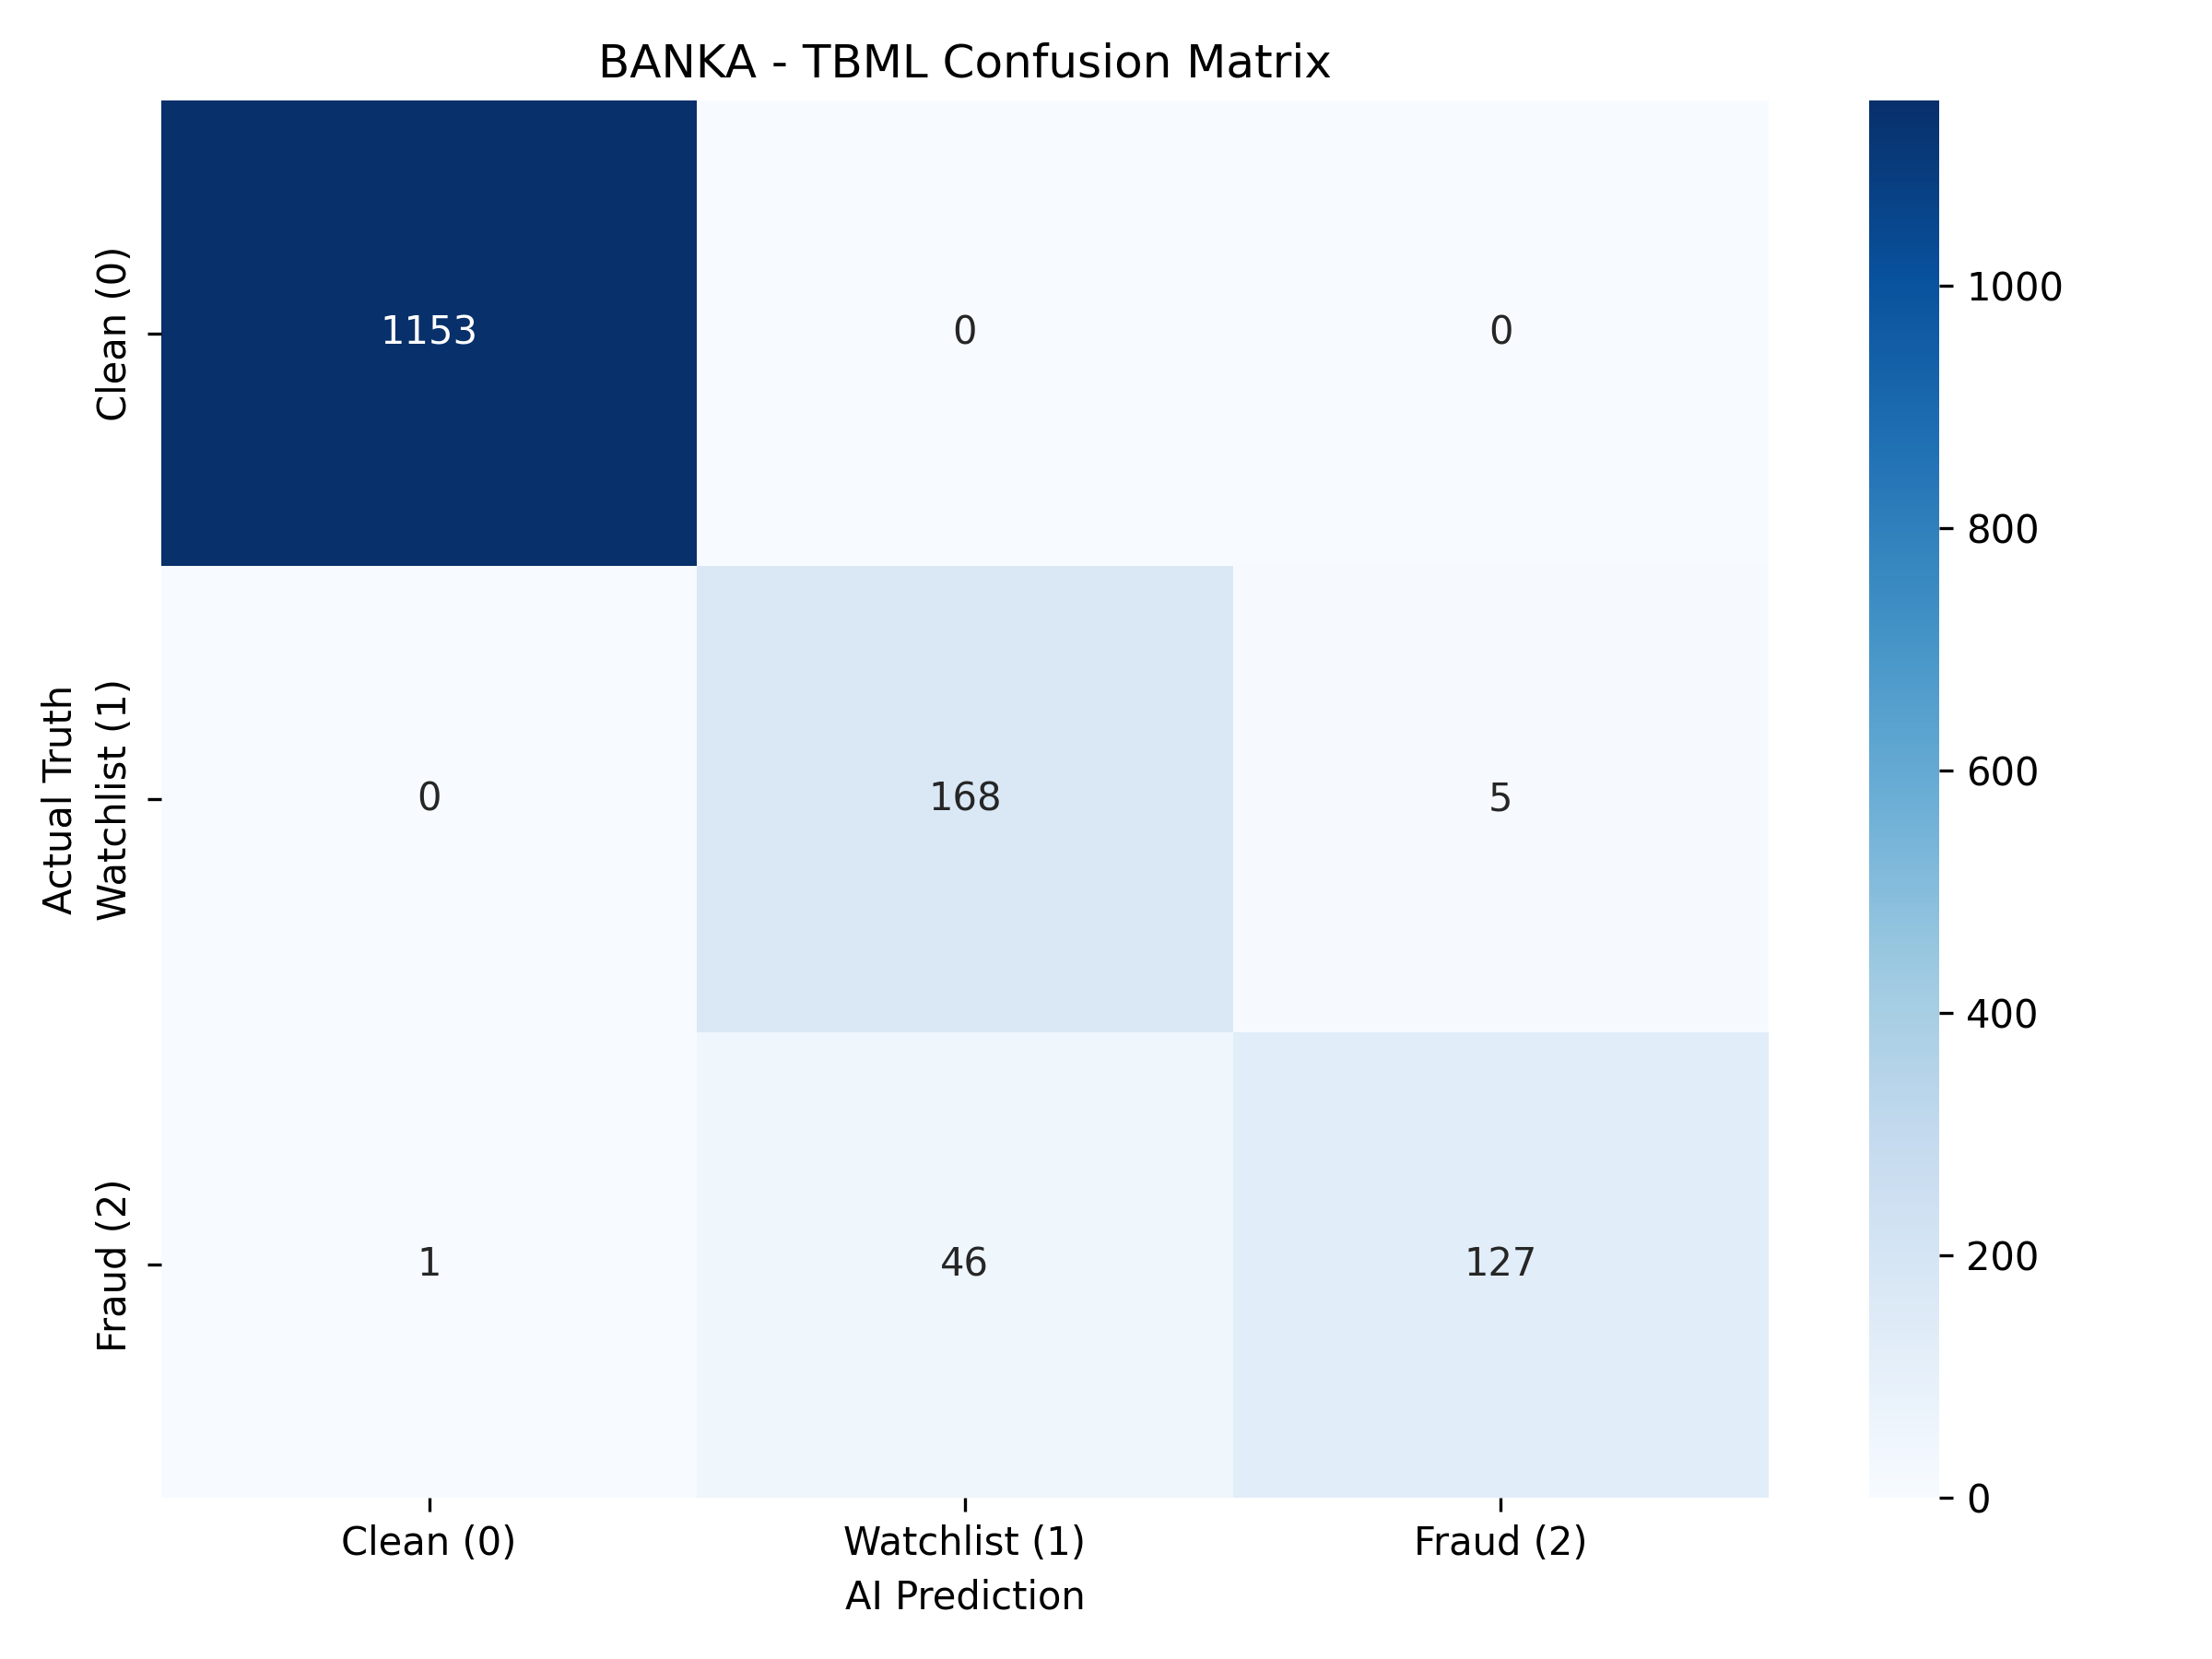
\includegraphics[width=\linewidth]{Figures/banka_confusion_matrix_deep.png}
\end{minipage}

\caption{BANKA Precision--Recall Curve and Confusion Matrix Validation}
\label{fig:banka_validation}
\end{figure}

As illustrated in Figure~\ref{fig:banka_validation}, the institutional environment of BANKA showed a highly
effective fraud-classification capacity, as measured by the Precision-Recall curve,
wherein the calculated Average Precision (AP) value amounted to about 0.92. The
curve showed highly precise detection at various levels of recall, reflecting an efficient
identification of the fraudulent transactional behavior even under class-imbalanced operational conditions. Additionally, the classification of Clean transactions proved perfect, as
no false positives were observed, and none of the transactions of this category was misclassified as fraud. Similarly, the classification of Watchlist transactions also showed a
high level of effectiveness, except for some instances that were classified as Fraud. In
addition, there was significant overlap between Fraud and Watchlist transactions,
where some of the transactions of the former category were classified as suspicious.
Nevertheless, the model kept its fraud-detection efficiency intact.

%--------------------------------------------------------
\subsection{BANKB Precision--Recall and Confusion Matrix Validation}
%--------------------------------------------------------

\begin{figure}[H]
\centering

\begin{minipage}{0.48\textwidth}
\centering
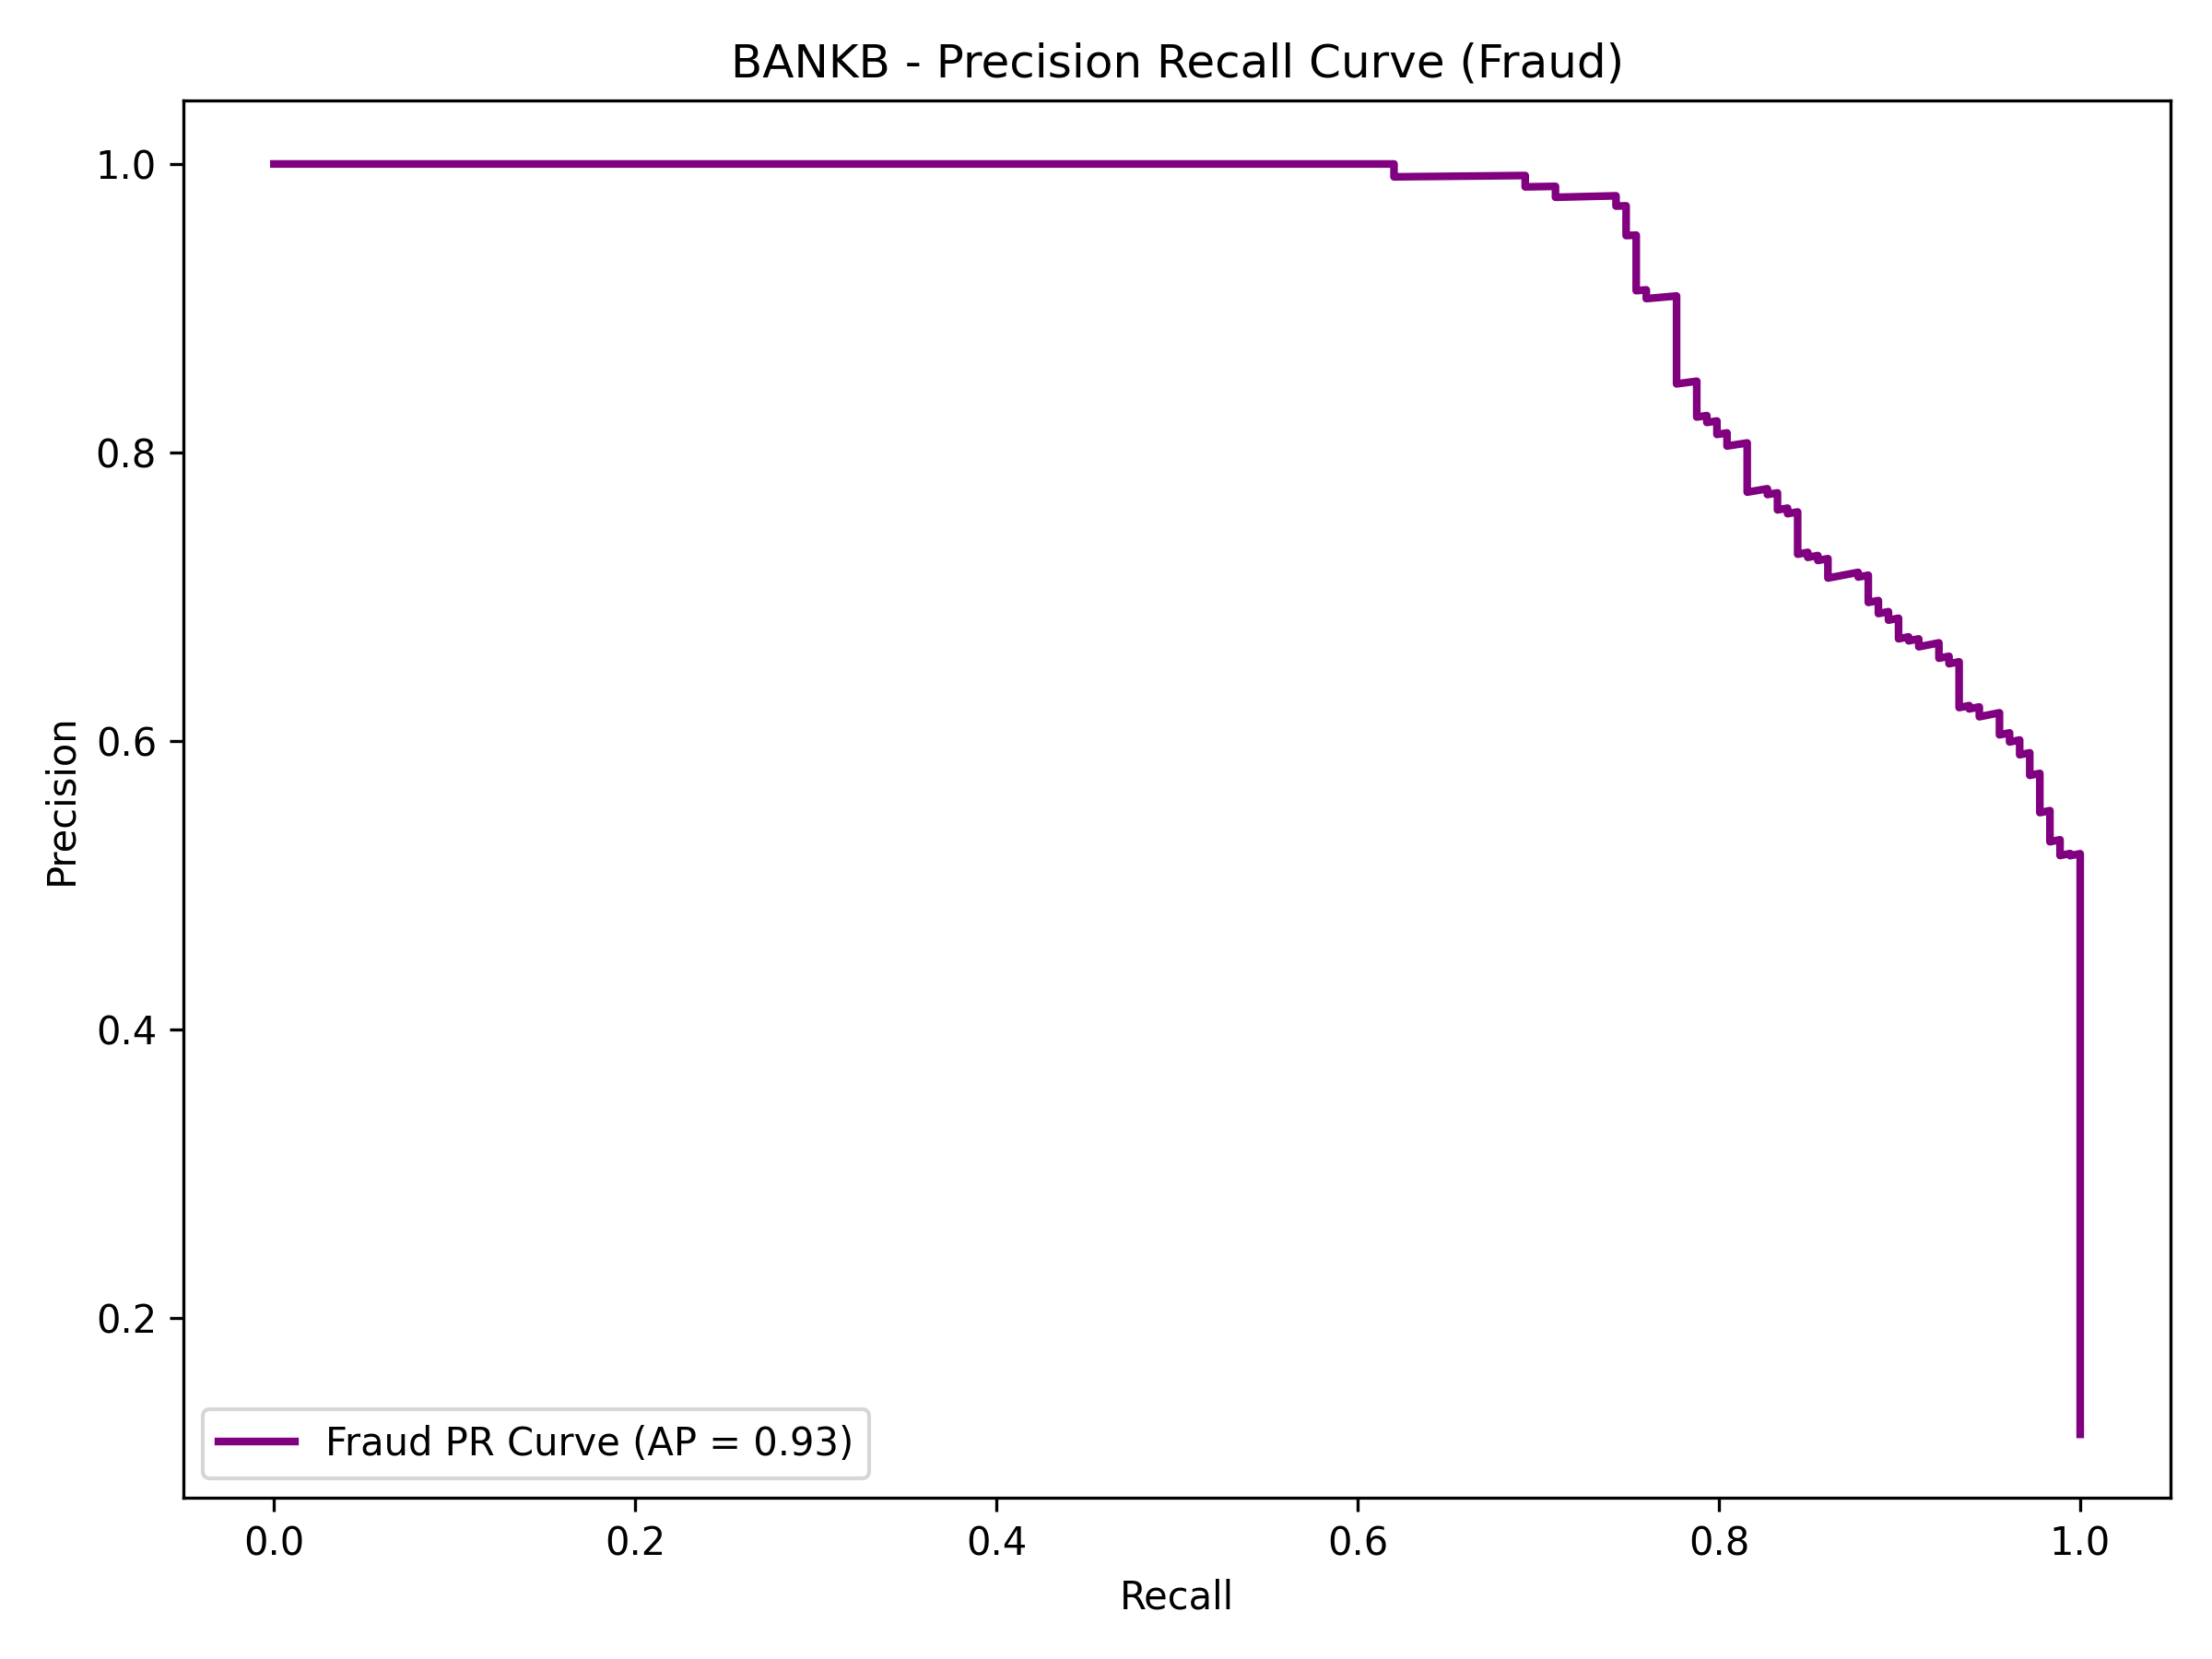
\includegraphics[width=\linewidth]{Figures/bankb_pr_curve_deep.png}
\end{minipage}
\hfill
\begin{minipage}{0.48\textwidth}
\centering
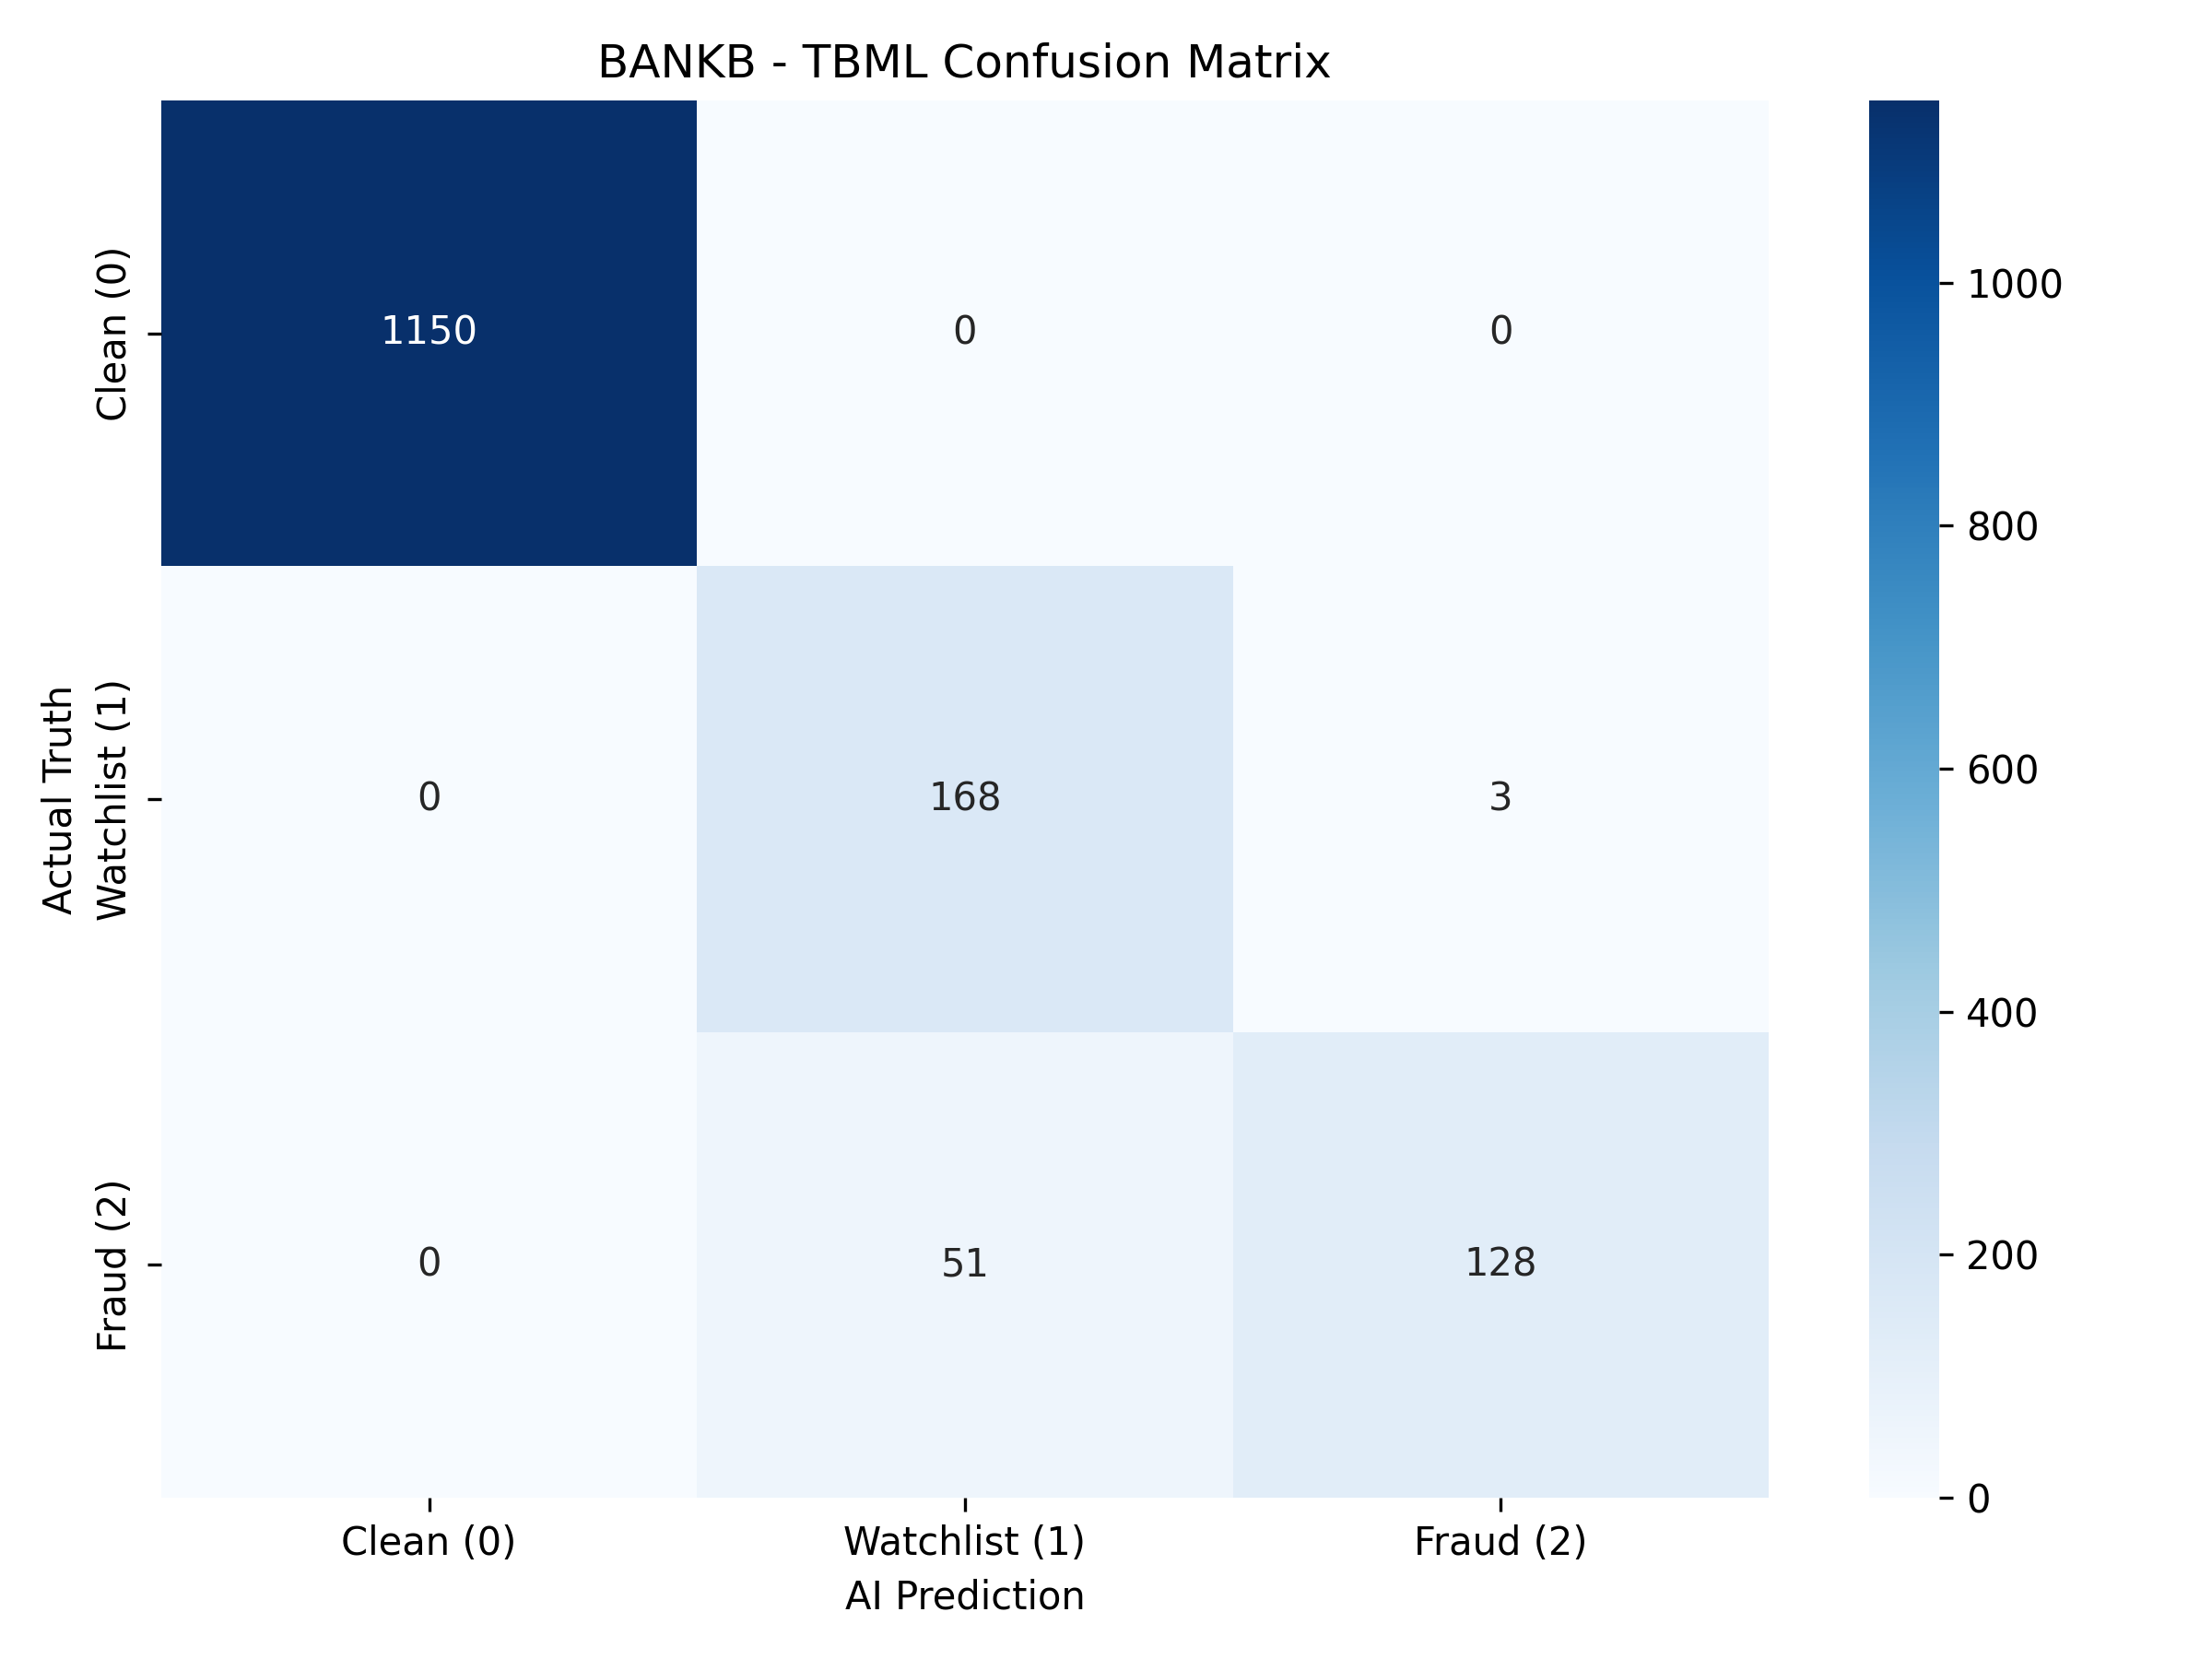
\includegraphics[width=\linewidth]{Figures/bankb_confusion_matrix_deep.png}
\end{minipage}

\caption{BANKB Precision--Recall Curve and Confusion Matrix Validation}
\label{fig:bankb_validation}
\end{figure}

As illustrated in Figure~\ref{fig:bankb_validation}, there was good fraud-classification ability within
the operational institutional environment of BANKB, because the generated Precision–Recall
curve resulted in a score of Average Precision (AP) that was equal to around 0.93.
The curve had kept high levels of precision for a wide range of the recall values,
thus, reflecting successful identification of fraud under conditions of class imbalance.
In its turn, the confusion matrix reflected excellent performance by showing perfectly
clean transaction class identification without making any false clean-to-fraud classification
errors. Transactions marked as "watchlist" were classified with high precision, while
only a few cases were mistakenly put into the Fraud class. As for the classification
overlap, it happened only for Fraud and Watchlist transaction classes, where some
transactions were classified as suspicious transactions. In spite of the overlap, fraud
detection ability remained sufficiently high. 



%========================================================
\subsection{BANKC Precision--Recall and Confusion Matrix Validation}
%--------------------------------------------------------

\begin{figure}[H]
\centering

\begin{minipage}{0.48\textwidth}
\centering
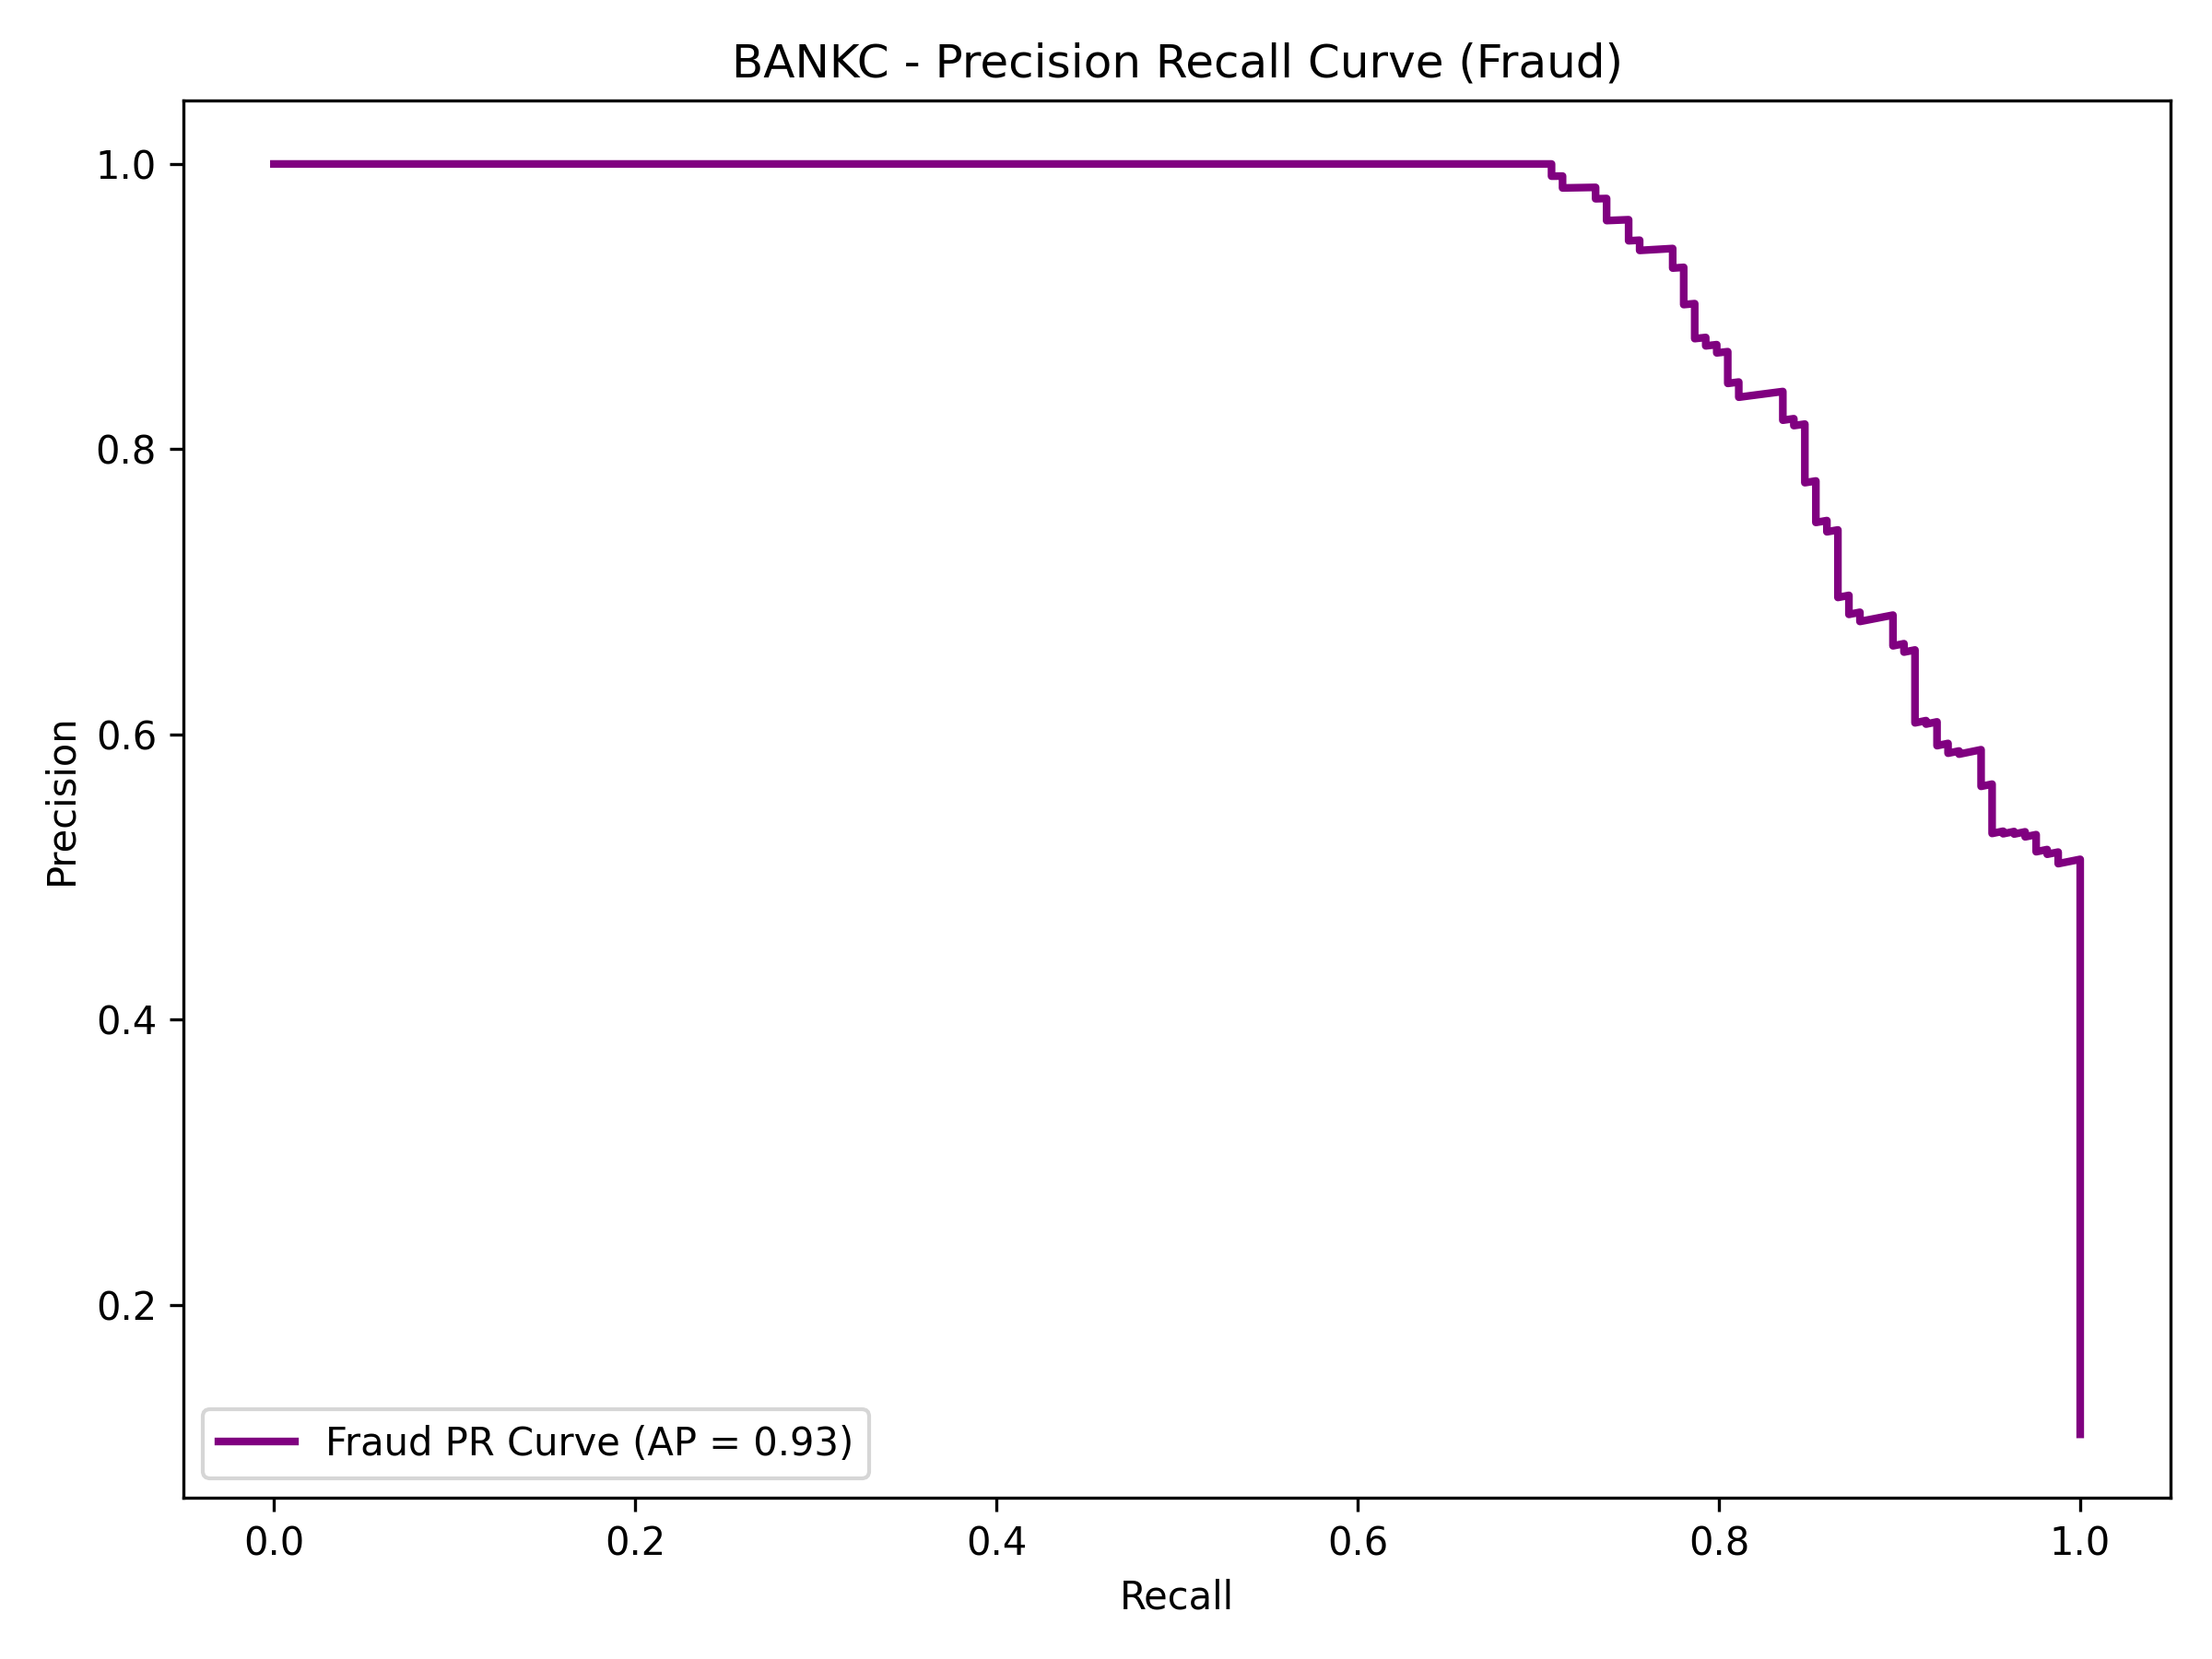
\includegraphics[width=\linewidth]{Figures/bankc_pr_curve_deep.png}
\end{minipage}
\hfill
\begin{minipage}{0.48\textwidth}
\centering
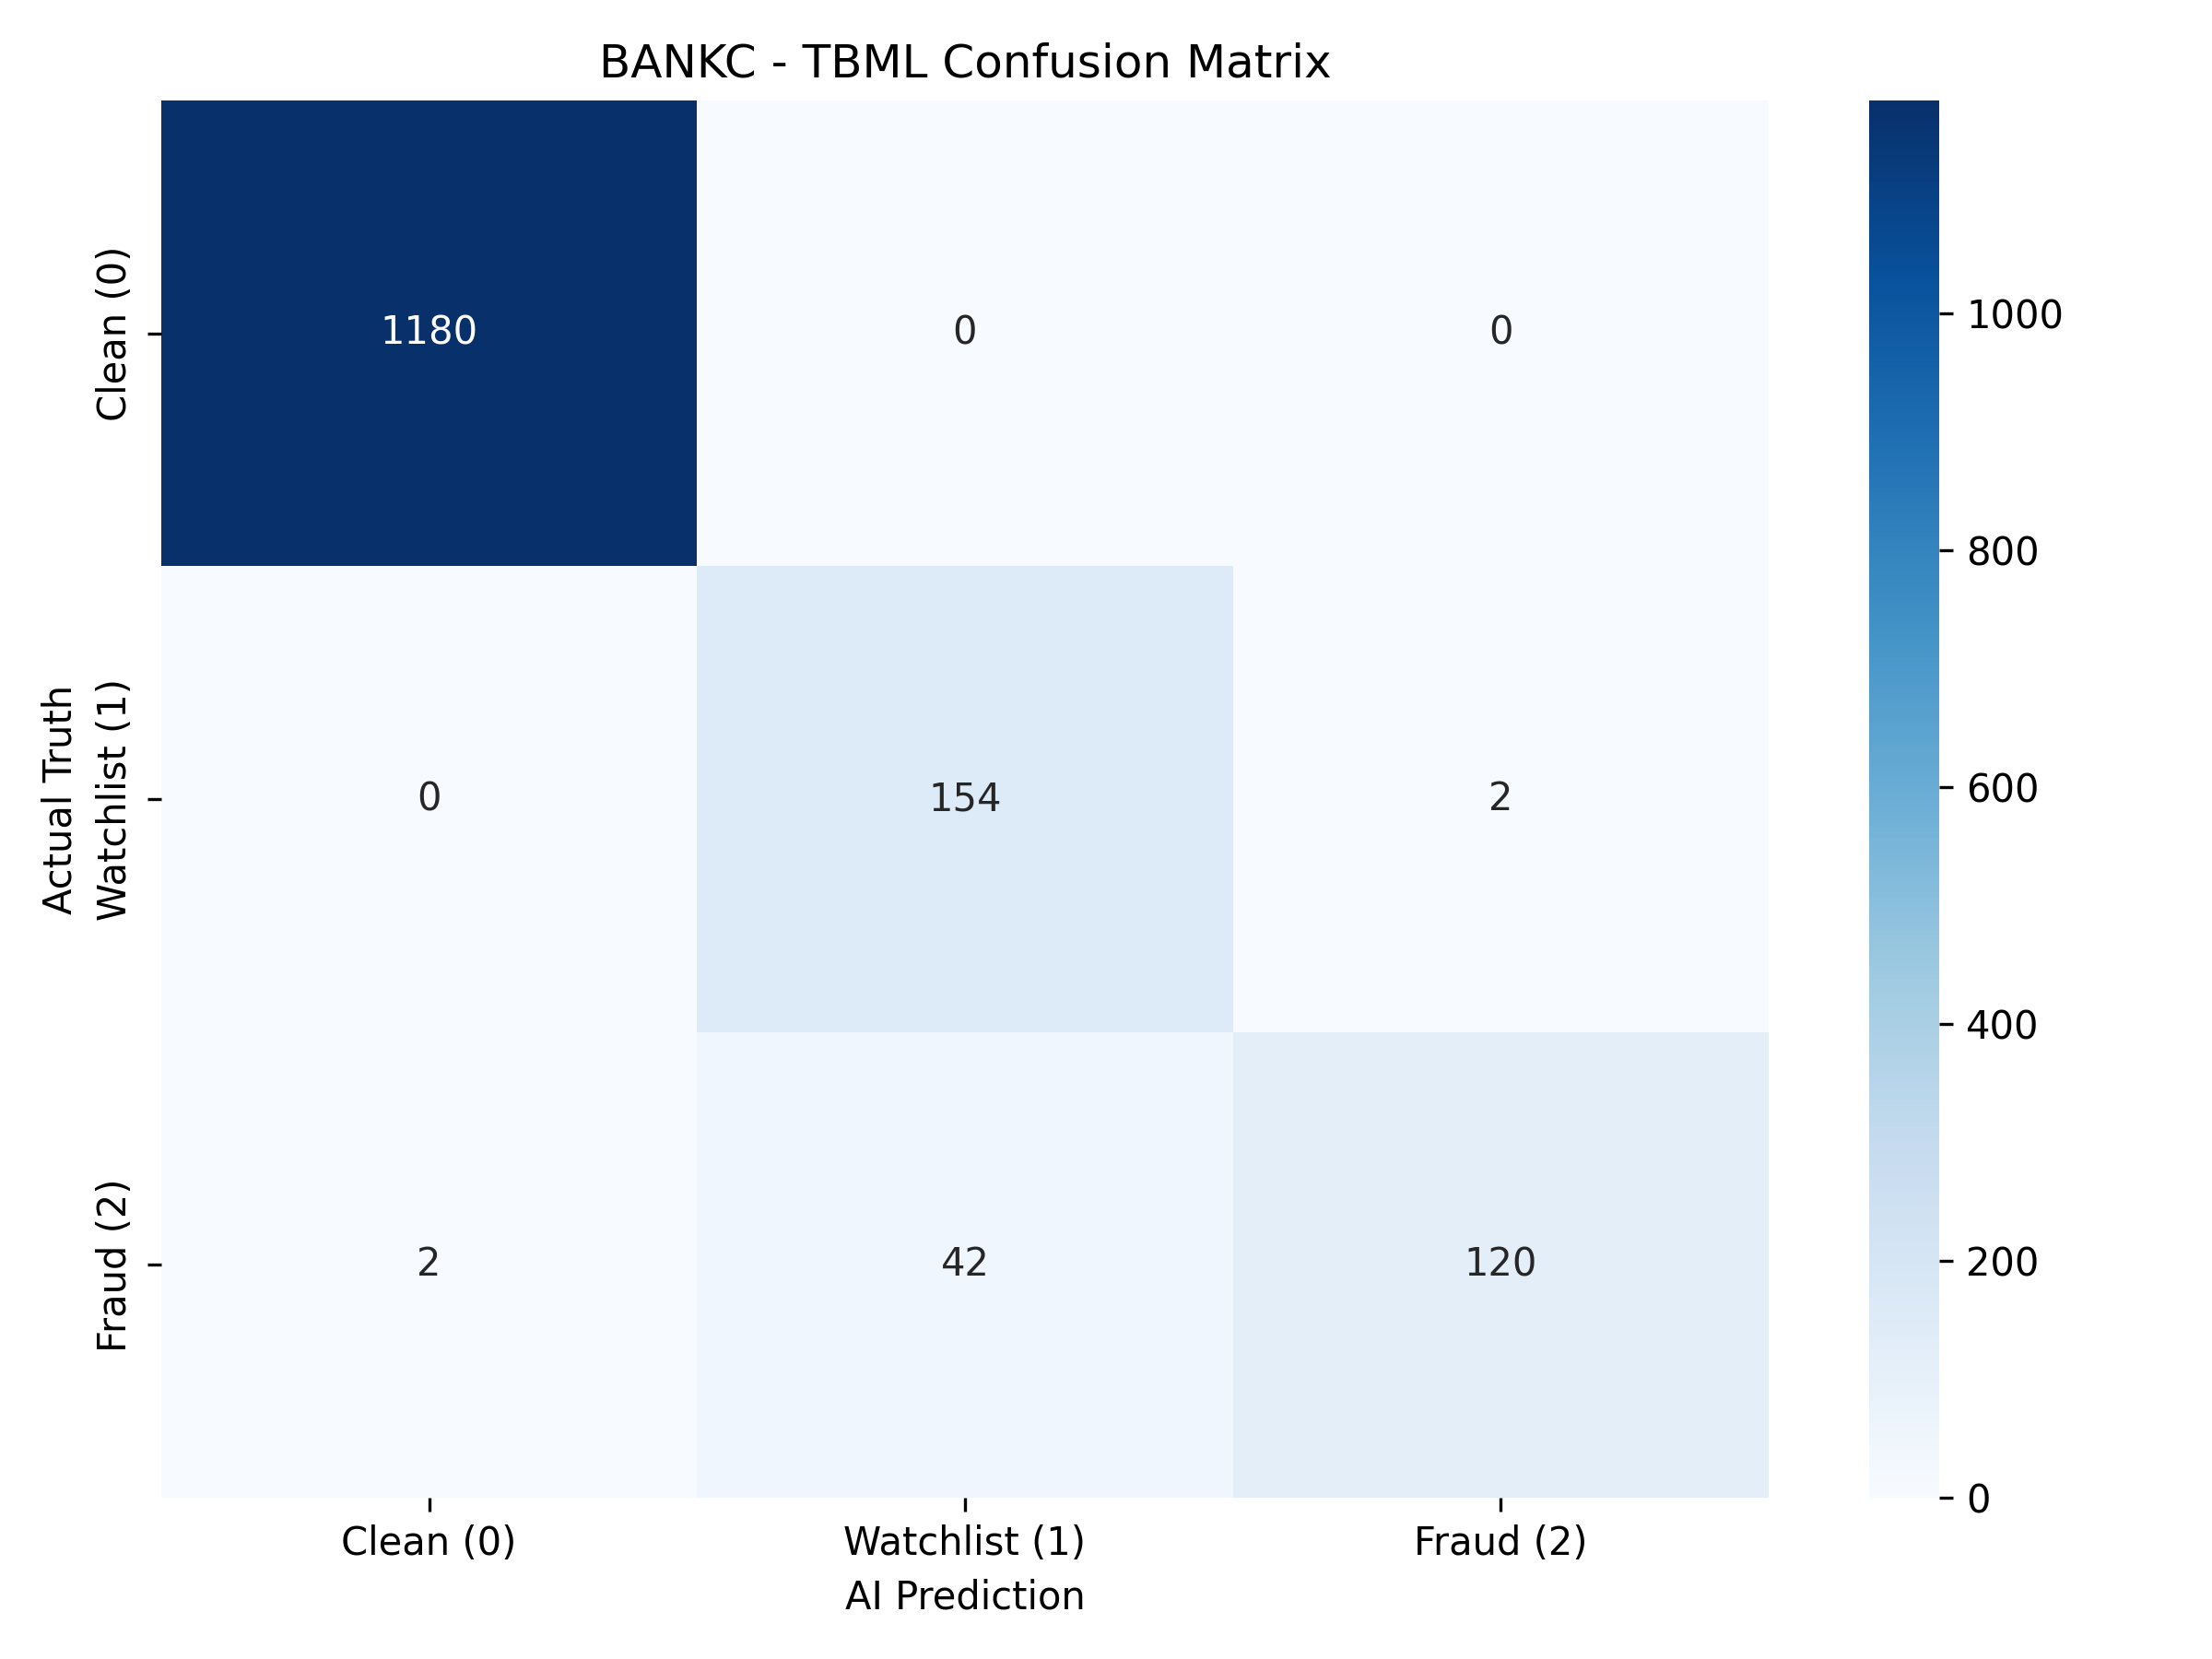
\includegraphics[width=\linewidth]{Figures/bankc_confusion_matrix_deep.png}
\end{minipage}

\caption{BANKC Precision--Recall Curve and Confusion Matrix Validation}
\label{fig:bankc_validation}
\end{figure}

As illustrated in Figure~\ref{fig:bankc_validation}, 
the precision-recall analysis shows that the BANKC
institutional environment exhibited great success in terms of classification of fraudulent
transactions, with the obtained Average Precision (AP) value amounting to roughly 0.93.
Furthermore, the graph showed excellent precision for various levels of recall, which is
indicative of the ability to detect fraudulent transactions under conditions of imbalanced
operating class environments. Additionally, perfect results for clean transactions can be
noted, as well as correct assignment of all suspicious transactions into their respective
transaction categories with no clean-to-fraud transactions. Finally, although there was
overlapping classification between watchlist and fraud categories (with some fraudulent
activities recognized as suspicious), the model successfully distinguished between the three
types of transactions in question.


\newpage
%========================================================
\section[Summary]{\textbf{Summary}}
%========================================================

This chapter validated the frameworks operational stability, synchronization reliability, and scalability across distributed institutional environments. Testing confirmed robust backend and graph-processing integration, secure transactional synchronization, and consistent dashboard performance under load. Model evaluation demonstrated strong multi-class discrimination, stable federated convergence, and reliable detection of suspicious and fraudulent transactions. The next chapter presents the detailed results and discussion.
